%\linenumbers*
%\chapter{OBSERVED RAINFALL CHARACTERISTICS OF THE STUDY AREA}
\section{Observed Rainfall Characteristics Of The Study Area}
\label{sec:RainfallCharacteristicsOfTheStudyArea}

%This chapter should really focus on comparing observed intensity trends with
%what is predicted for the future---not \emph{just} looking at trends, but
%seeing how well those trends are consistent with, or different from, GCM
%predictions for the future. You should mention that here.

\subsection{Introduction}
\label{sec:ObservedRainfallIntroduction}
%******In this chapter, why observed data were analysed is to be explained.
%Also, I need to indicate what are the possible benefits taking this route
%rather than other ways such as downscaling or perturb with GCM (or RCM)
%outputs.
As stated previously, it became apparent at the early stage of this research
that RCM rainfall data could not (and still cannot) be used directly for erosion
simulations. Although RCMs and empirically downscaled data from GCMs allow
projections to be made at a finer scale than GCMs, RCM projections still vary
greatly between models in the same way as GCMs and empirical downscaling does
not attempt to correct any biases in the data from the GCMs. Even with a finer
scale than GCMs, RCM data do not hold sufficiently detailed information of
rainfall intensity that can be used directly for erosion simulations, and were
not reliable enough for this type of approach yet---and still they are not
\citep{nearing2001-229,michael2005-155,o'neal2005-165}. That is why this part of
research was carried out.

Moreover, using outputs from a model as inputs to another model will increase
the level of uncertainty because there may be compound errors originated from
both models. For example, when RCMs generate future rainfall data, these
rainfall data are in a wrong scale, that is a larger scale than what is needed
for erosion simulations. Also, rainfall intensity data that have been obtained
from these RCM-generated rainfall data will be in a wrong scale. This scale
mis-match induces the use of downscaling to make the data usable for soil
erosion modelling. During these processes, the level of uncertainty will
increase process after process. Therefore, using observed rainfall data for
erosion simulations may be more beneficial than using RCM data. It certainly is
easier to track errors from known sources such as observed rainfall data, too.

The limitation of using observed data would be that it needs correctly scaled
data to begin with and needs reasonably long data duration to be able to pick up
seasonal variations at least, if not greater. Also, it should be remarked that
this approach is to create scenarios of future rainfall which are based on
present-day rainfall, not future rainfall. Thus, this approach assume that
future rainfall trends stay the same as present-day rainfall trends.
%Is the future rainfall intensity going to be different from the present? If so,
%how is it going to be different? Is it going to increase---or decrease?

In this chapter, three different scales of observed rainfall records were
analysed to find the rainfall intensity trend---Monthly 0.5\textdegree\ grid
rainfall, daily station rainfall and event rainfall measured by tipping-bucket
gauges. The descriptions of these data are covered in Section \ref{sec:Data}.

\subsection{Method}
\label{sec:MethodsObservedRainfallCharacteristicInvestigation}
%(***REFS NEEDED to back this up, for example, refs that used observation to
%estimate trends and method I used.) %(***NOTE TO SELF Emphasise that it has
%been done before and proven, also say about pros and cons. in discussion)
All three datasets described previously (Table
\ref{tab:PrecipitationDataUsedForCurrentRainfallTrendInvestigation}) were
analysed to find out rainfall intensity trends in the area using simple linear
regression and Mann-Kendall (M-K) rank correlation. Monthly 0.5\textdegree\ grid
rainfall data and daily station rainfall data were used without any conversion.
Event rainfall data recorded by a tipping-bucket gauge are analysed.
Tipping-bucket gauge rainfall data were aggregated into 1-min rainfall data
prior to use. Rainfall amount, duration and daily maximum 1-min peak intensity
were investigated using 1-min event rainfall data.

\citet{kundzewicz2004-7} suggested a number of tests for trend detection:
Spearman's rho, Kendall's tau/Mann-Kendall test, Seasonal Kendall test, Linear
regression and other robust regression tests.
\citet{hannaford2006-1237} also used three methods (i.e.\ M-K rank, Spearman's
rho and linear regression) to assess trends in UK runoff and low flows. They
found a good agreement between the detection rate of trends between the three
trend-testing methods.
More studies have observed a high degree of equivalence between M-K rank and
Spearman's rho tests \citep{yue2002-254} and M-K rank and linear regression
\citep{svensson2005-811}

\citet{yue2002-254} investigated the power of M-K rank and Spearman's rho. They
found that both have similar power in detecting a trend to the point of being
indistinguishable in practice. \citet{yue2002-254} said ``The power of M-K rank
test depends on the pre-assigned significance level, magnitude of trend, sample
size, and the amount of variation within a time series. That is, the bigger the
absolute magnitude of trend, the more powerful are the tests; as the sample size
increases, the tests become more powerful; and as the amount of variation
increases within a time series, the power of the tests decrease. When a trend is
present, the power is also dependent on the distribution type and skewness of
the time series.''

Thus, two trend test methods, that are linear regression and M-K rank, are used
in this section.

The trends in daily rainfall characteristics were investigated. Rainfall related
indicators were calculated to determine rainfall characteristics (Table
\ref{tab:RainfallIntensityIndicators}). Daily rainfall intensity is obtained by
dividing the monthly rainfall amount by the number of raindays.

\begin{table}[htbp]
  \figureversion{tabular}
  \centering
  \caption{Rainfall intensity indicators}
  \label{tab:RainfallIntensityIndicators}
  \footnotesize
    \begin{tabular}{l p{95mm} l}
    \toprule
    \textbf{Indicator} & \textbf{Definition} & \textbf{Unit}\\
    \midrule
    RR & Precipitation sum & mm\\
    RR1 & Number of wet days (RR $\geq$ 1 mm/day) & days\\
    SDII & Simple daily intensity index: \[\frac{\textrm{total
rainfall amount for wet days (RR $\geq$ 1 mm/day)}}{\textrm{number of wet days}}
\] & mm/day\\
    %\addlinespace[-2.5mm]
    R10mm & No. of days with precipitation $\geq$ 10 mm/day & days\\
    R20mm & No. of days with precipitation $\geq$ 20 mm/day & days\\
    R10p$^\dagger$ & Ratio of days with precipitation $\geq$ 10
mm/day ((R10/RR1)$\times100$) & \%\\
    R20p$^\dagger$ & Ratio of days with precipitation $\geq$ 20
mm/day ((R20/RR1)$\times100$) & \%\\
    \bottomrule
%   \addlinespace[1mm]
    \multicolumn{3}{p{12cm}}{\footnotesize $^\dagger$\ Additional
indicators, which are not listed in the European Climate Assessment \& Dataset
project (ECA\&D) website. Complete list of indicators and their definitions are
available at http://eca.knmi.nl/indicesextremes/indicesdictionary.php}
    \end{tabular}
\end{table}

Any year with partial records were discarded to minimize the effects from
missing data (Table \ref{tab:DailyRainfallStationsAndRecordDetails}).
The records of the last year of each station were also discarded as they are
incomplete. For example, daily rainfall data from Falmer Farm (FF) were
considered only for 1904--1996 discarding the records for 1997 and 1999 with
missing data. Three more years (1998, 2000 and 2001) were discarded from all the
stations because of the discontinuity resulted in by removing missing data
periods. Also, there was a problem with 2000 rainfall because they were recorded
as weekly total rather than daily total.

\begin{table}[htbp]
  \figureversion{tabular}
  \centering
  \caption{Daily Rainfall Stations and Record Details }
  \label{tab:DailyRainfallStationsAndRecordDetails}
  \small
    \begin{tabular}{llll} \toprule
    \textbf{Code} & \textbf{Station Name} & \textbf{Periods}* &
\textbf{Studied Periods}*\\
    \midrule
    DR & Ditchling Road & 1980--1989 (10) & 1980--1988 (9)\\
    SO & Southover & 1980--1998 (19) & 1980--1997 (18)\\
    PL & Plumpton & 1980--2000 (21) & 1980--1998 (19)\\
    PB & Poverty Bottom & 1980--1998 (19) & 1980--1997 (18)\\
    SDR & Seaford D. Road & 1980--2000 (21) & 1980--1999 (20)\\
    EW & Eastbourne Wilmington & 1980--2000 (21) & 1980--1999 (20)\\
    FT & Friston Tower & 1980--2000 (21) & 1980--1999 (20)\\
    LI & Litlington & 1980--2000 (21) & 1980--1999 (20)\\
    HPF & High Park Farm & 1974--2004 (31) & 1975--2003 (29)\\
    HD & Housedean & 1967--2004 (39) & 1968--2003 (37)\\
    FF & Falmer Farm & 1904--2002 (99) & 1904--1996 (93)\\
    \bottomrule
    %\addlinespace[1mm]
    \multicolumn{4}{l}{\footnotesize * (\ ): Number of years}
    \end{tabular}
\end{table}

There are some missing data periods for event data from Ditchling Road (DR) and
Southover (SO) as well. All the years with any missing data period was
discarded. Thus, only 9, 4 and 2 year-long data were used from Ditchling Road
(DR), Southover (SO) and Plumpton (PL) stations, respectively.

In this research, daily rainfall is defined as the total rainfall that fell in a
24-hour period beginning at 9:00 am, and the day is indicated by the date on
which the period begins. For example, precipitation of 5.2 mm on 29 July 2001
means that the cumulative amount of precipitation between 9:00 am, 29 July 2001
and 9:00 am, 30 July 2001 was 5.2 mm. A ``midnight to midnight'' approach is
rarely used for rainfall data records because of practical difficulties for
observation. British Summer Time (BST) is not considered here. A wet day is also
defined when the amount of daily precipitation is equal to or more than 0.2 mm.

All no-rain periods within a day were removed from 1-min event rainfall data,
and rainfall durations were calculated as effective durations. It has been
assumed that there is only one storm on a given wet day, and rainfall is
continuous during that storm. This approach was used for CLIGEN to parametrise
daily rainfall storm. Rainfall intensity was calculated by dividing rainfall
amount by the effective duration.

\subsection{Monthly Precipitation}
\label{sec:HalfDegreeGridMonthlyPrecipitationData}

Observed mean annual rainfall amount from the studied 0.5\textdegree\ grid
during 1901--2000 period is 902.6 mm.
Annual rainfall amount which is calculated from monthly grid data show no
significant trend (Figure \ref{fig:grid_annual_amount}).

\begin{figure}[htbp]
  \centering
    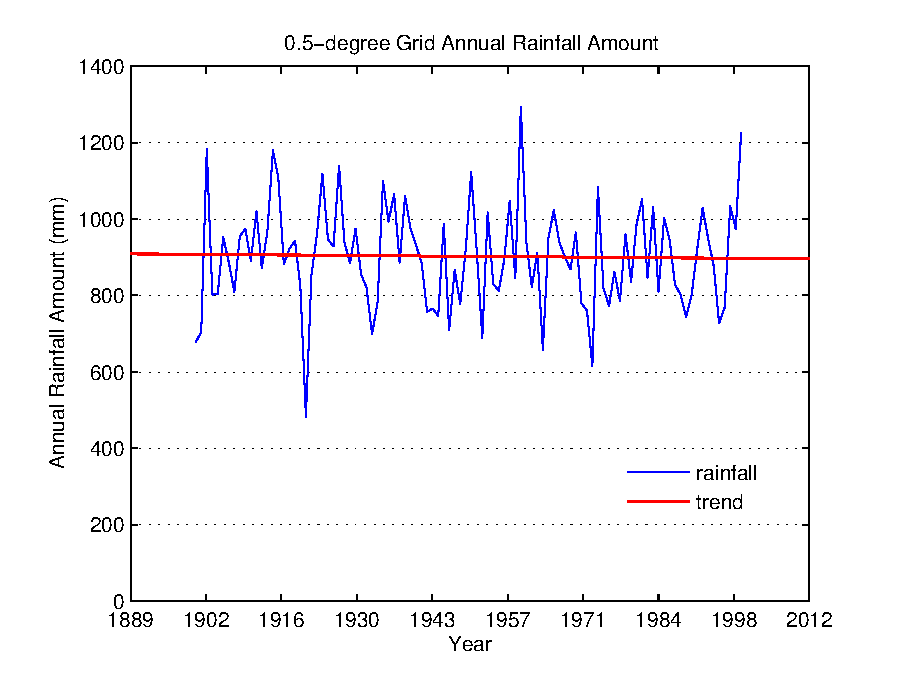
\includegraphics[width=0.7\textwidth]{./img/grid_annual_amount}
  \caption{Annual rainfall amount trend of monthly grid data}
  \label{fig:grid_annual_amount}
\end{figure}

There is no statistically significant trend in seasonal rainfall amounts
(Figure \ref{fig:grid_DJF_trend}).

\begin{figure}[htbp]
  \centering
    \subfloat[][DJF]{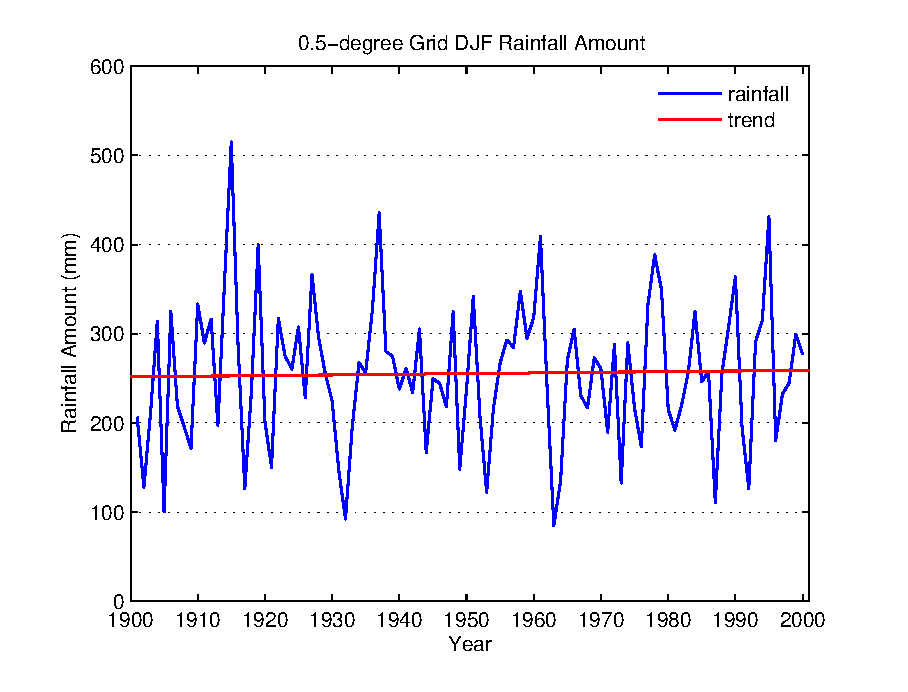
\includegraphics[width=0.5\textwidth]
{./img/grid_DJF_trend}}
    \subfloat[][MAM]{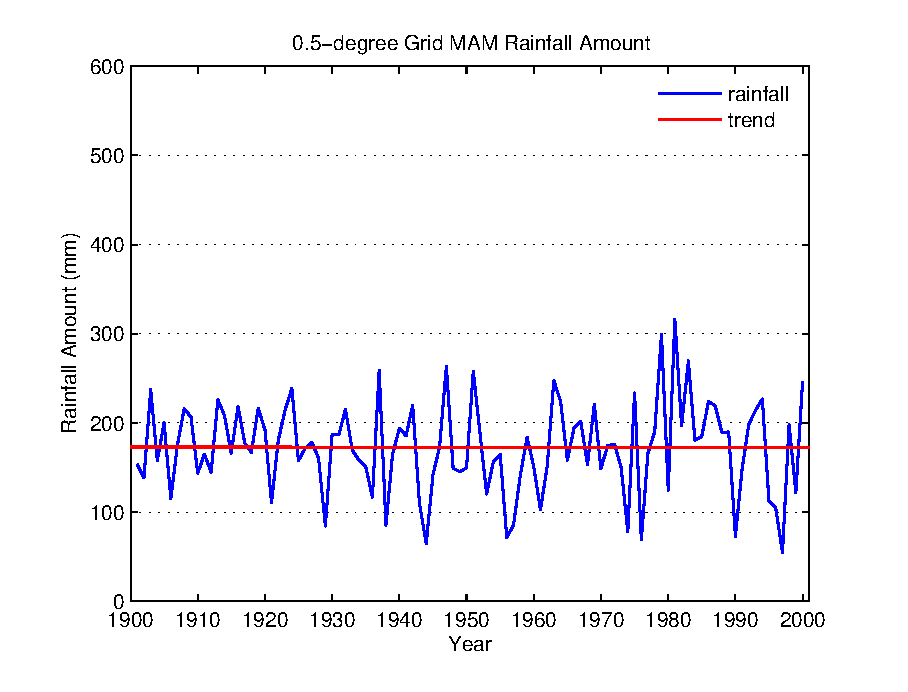
\includegraphics[width=0.5\textwidth]
{./img/grid_MAM_trend}}

    \subfloat[][JJA]{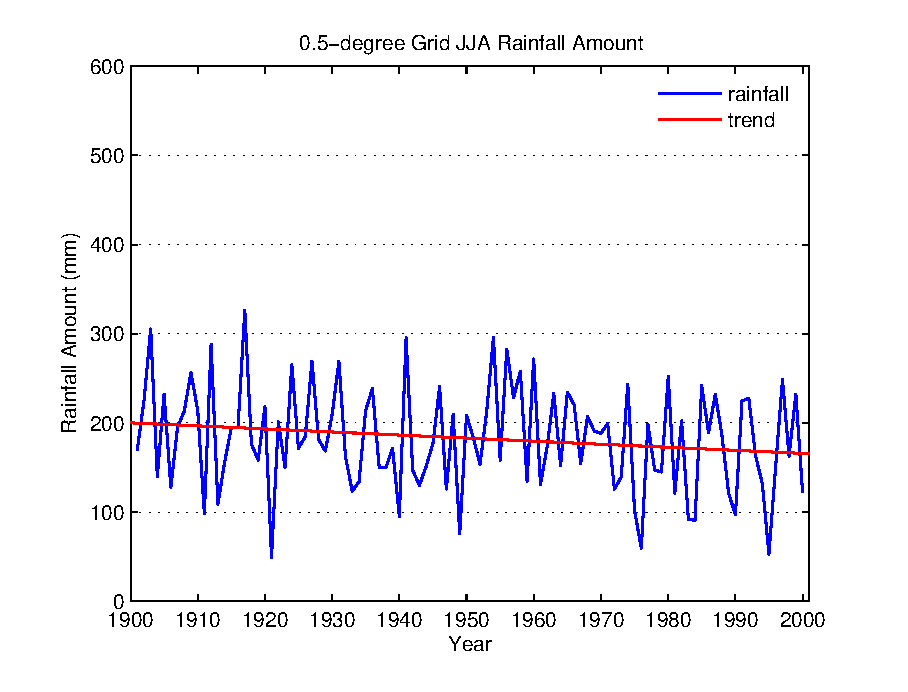
\includegraphics[width=0.5\textwidth]
{./img/grid_JJA_trend}}
    \subfloat[][SON]{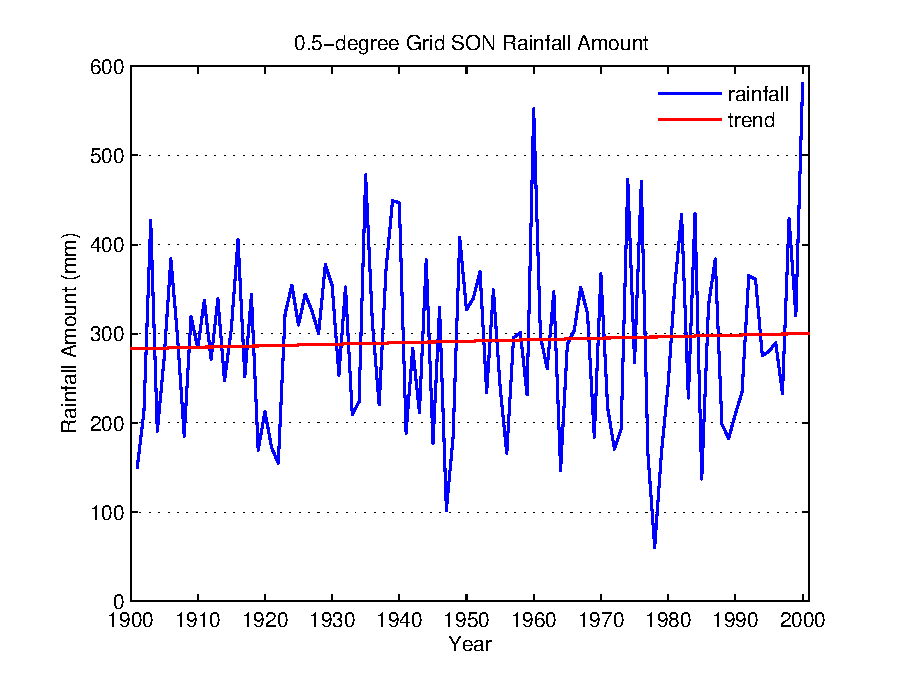
\includegraphics[width=0.5\textwidth]
{./img/grid_SON_trend}}
  \caption{Seasonal rainfall amount trend of monthly 0.5\textdegree\ grid
data}

  \label{fig:grid_DJF_trend}
\end{figure}

Monthly rainfall amount pattern shows more rainfall in autumn and winter months
with a peak in November, and less rainfall in spring and summer months (Figure
\ref{fig:grid_average_monthly}). Monthly analysis of the grid data shows more
detailed monthly trend in rainfall amount. Rainfall amounts in March show a
statistically significant ($p<0.05$) decreasing trend over 1981--2000 by both
simple linear regression and Mann-Kendall's test.

\begin{figure}[htbp]
  \centering
    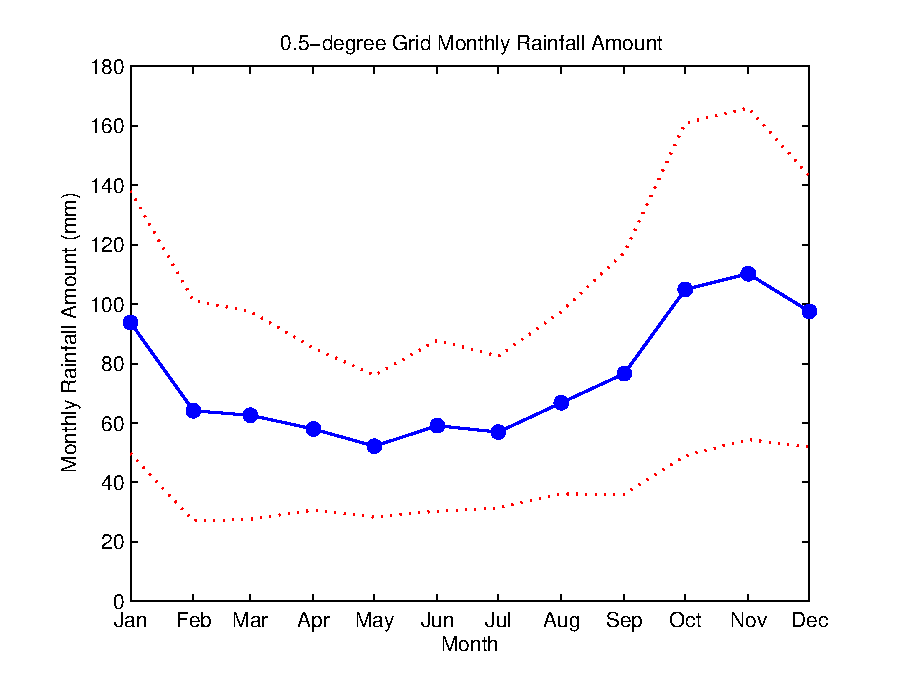
\includegraphics[width=0.7\textwidth]{./img/grid_average_monthly}
  \caption[Average monthly rainfall patterns of monthly grid data]{Average
monthly rainfall patterns of monthly grid data. Dotted lines indicate standard
deviation with 95\% confidence level.}
  \label{fig:grid_average_monthly}
\end{figure}

Rainfall amounts in July have a decreasing trend throughout the whole data
period (1901--2000) (Figure \ref{fig:grid_july_trend}).

\begin{figure}
  \centering
    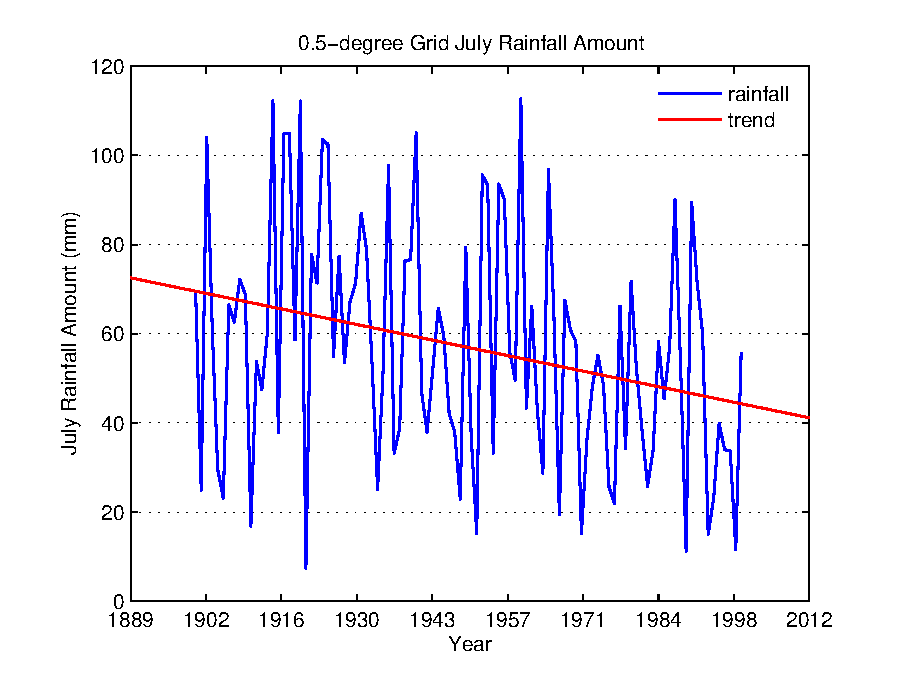
\includegraphics[width=0.7\textwidth]{./img/grid_july_trend}
  \caption{July rainfall amount trend over 1901-2000}
  \label{fig:grid_july_trend}
\end{figure}

%%%%%%%%%%%%%%%%%%%%%%%%%%%%%%%%%%%%%%%%%%%%%%%%%%%%%%%%%%
\subsection{Daily Precipitation}
\label{sec:DailyRainfallStationData}

Annual rainfall amount from Poverty Bottom (PB), Friston Tower (FT), Eastbourne
Wilmington (EW), Litlington (LI) and Seaford D. Road (SDR) stations are
significantly different from those of Plumpton (PL) or High Park Farm (HPF), for
example. This may be because of the distance from each other (see Figure
\ref{fig:DailyRainfallDataSite}) although all stations are placed in the
0.5\textdegree\ grid square.

%By stations, compare annual and monthly trend of rainfall amount and SDII.
%first of all, compare amounts for the Grid data. do this for annual and
%monthly. Are there July decrease and September increase in daily data too?
%if found and yes, it can be argued that SDII trends found in station daily
%data may be ture for the Grid Data.

\paragraph{Rainfall Amount (RR)}
\label{sec:RainfallAmountRR}

All the station show no statistically significant trend in annual rainfall
amount. This result agrees with that of monthly 0.5\textdegree\ grid rainfall
data.

For all the stations except Ditchling Road (DR), High Park Farm (HPF) and
Housedean (HD), monthly rainfall amount in March showed statistically
significant downward trends over the last two decades. The similar downward
trends are observed with rainfall amounts in July for the last decades with the
exception of DR, PB, HPF and HD stations. For longer periods, the trend of
monthly rainfall amount is inconclusive. This broadly agrees with the results
from the 0.5\textdegree\ grid data analysis. For monthly 0.5\textdegree\ grid
data, July months showed a decrease in rainfall amount.

\begin{figure}[htbp]
  \centering
  \subfloat[DR]{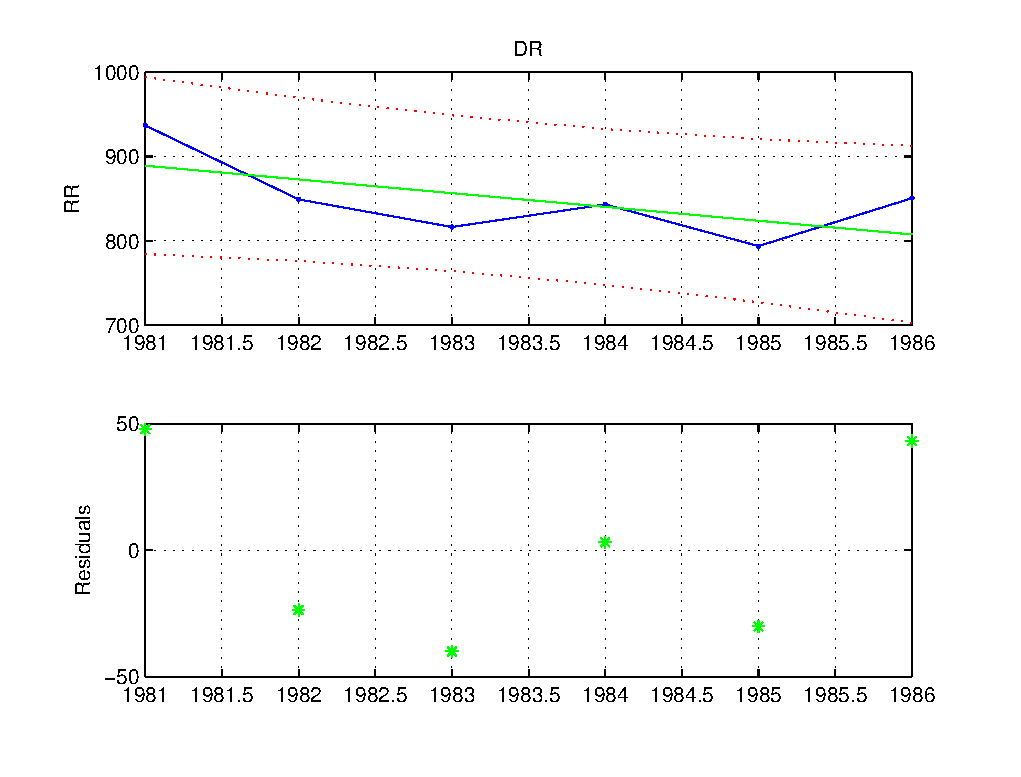
\includegraphics[width=0.33\textwidth]{./img/dr_rr}}
  \subfloat[SO]{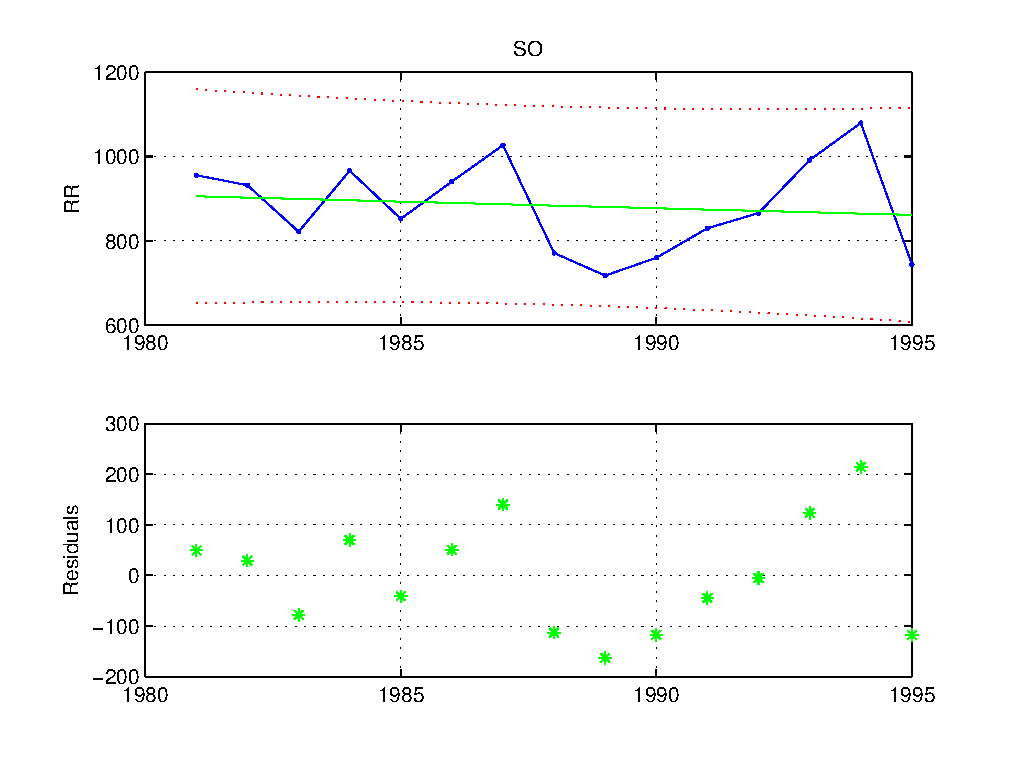
\includegraphics[width=0.33\textwidth]{./img/so_rr}}
  \subfloat[PL]{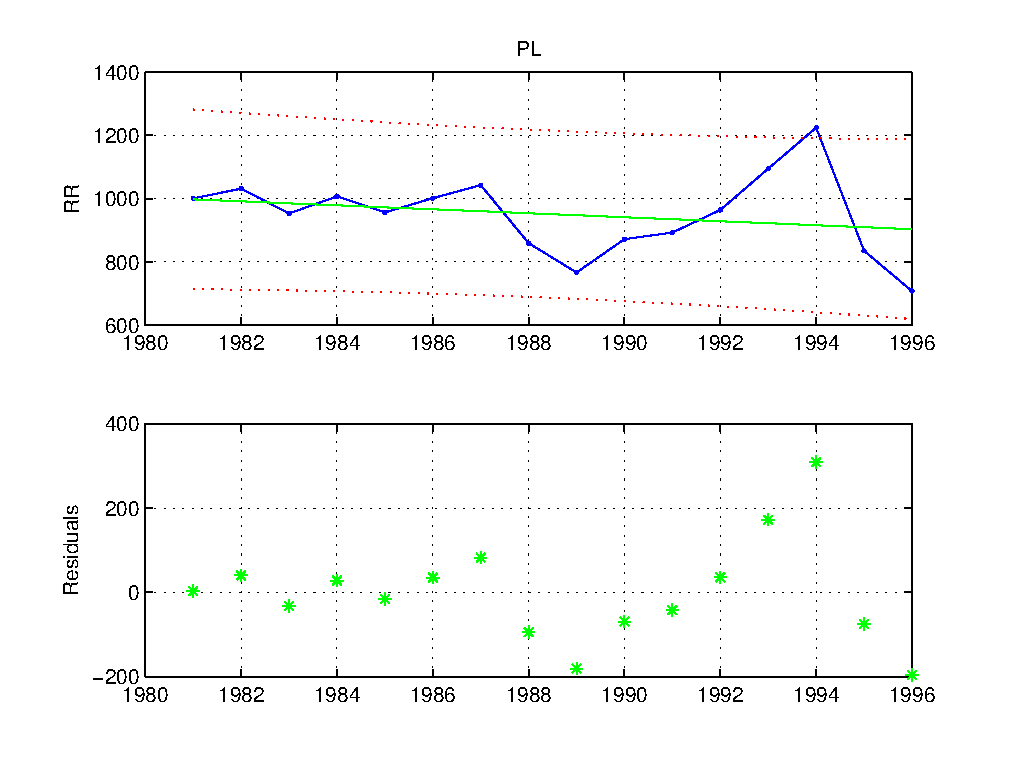
\includegraphics[width=0.33\textwidth]{./img/pl_rr}}

  \subfloat[PB]{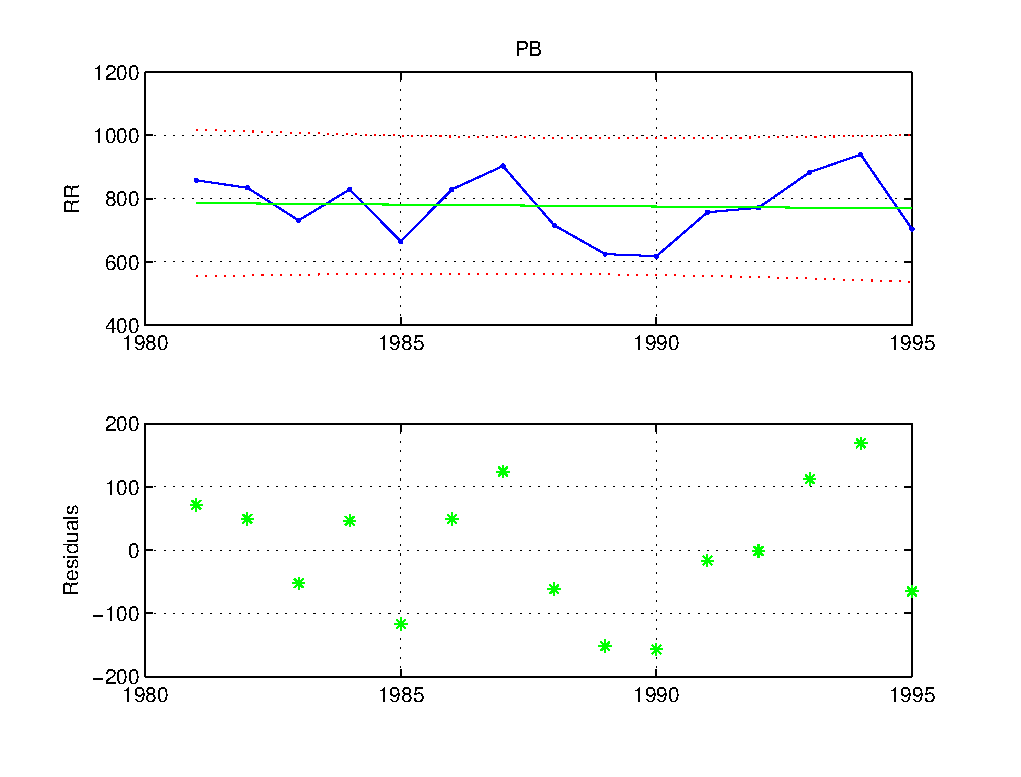
\includegraphics[width=0.33\textwidth]{./img/pb_rr}}
  \subfloat[SDR]{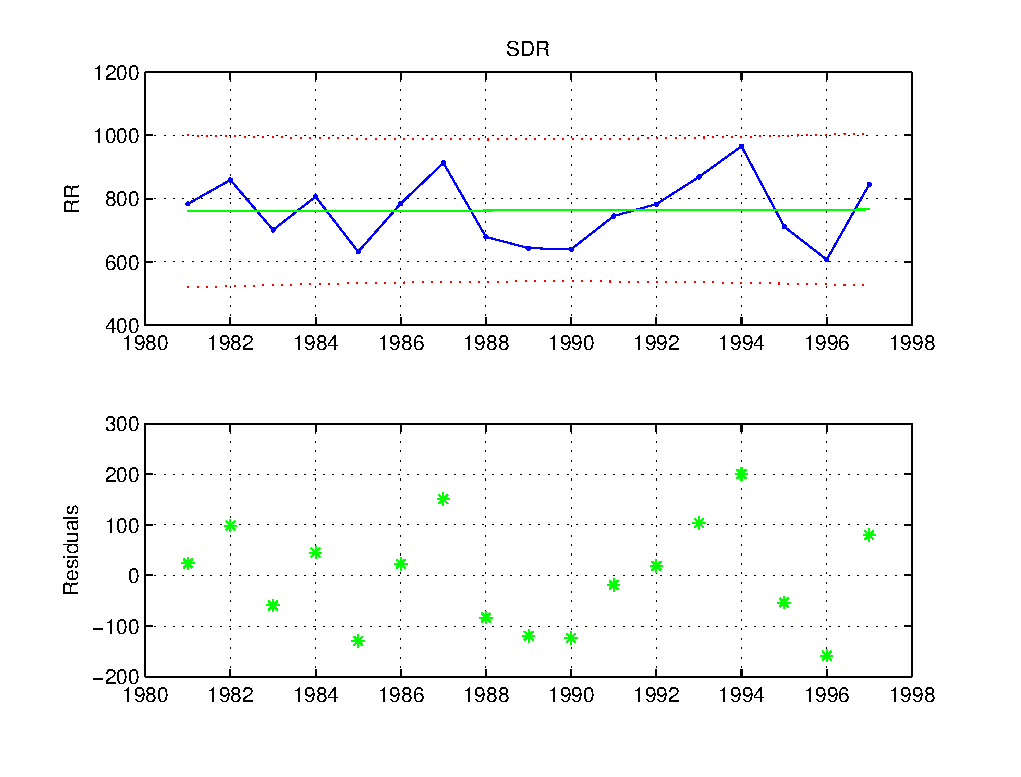
\includegraphics[width=0.33\textwidth]{./img/sdr_rr}}
  \subfloat[EW]{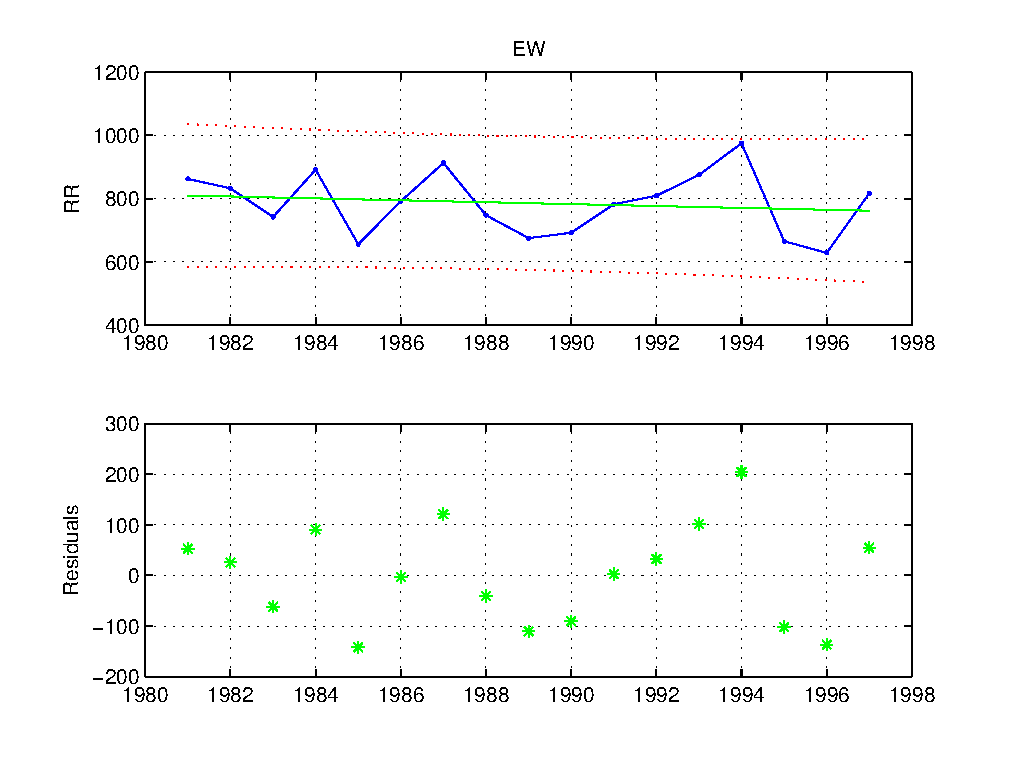
\includegraphics[width=0.33\textwidth]{./img/ew_rr}}

  \subfloat[FT]{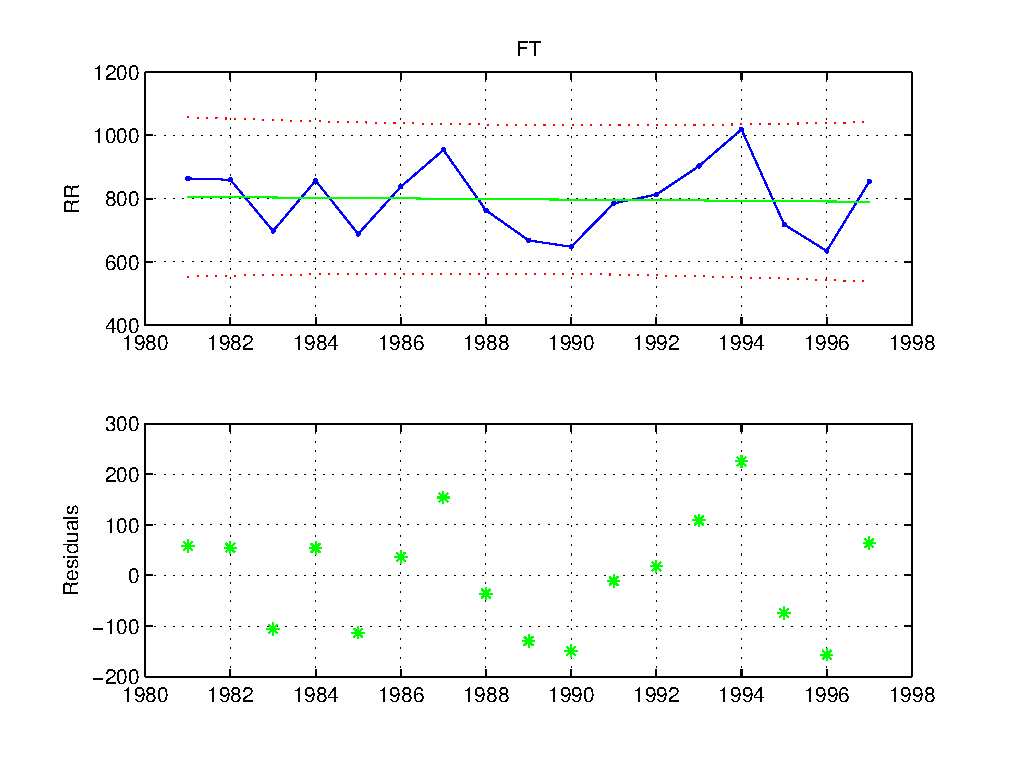
\includegraphics[width=0.33\textwidth]{./img/ft_rr}}
  \subfloat[LI]{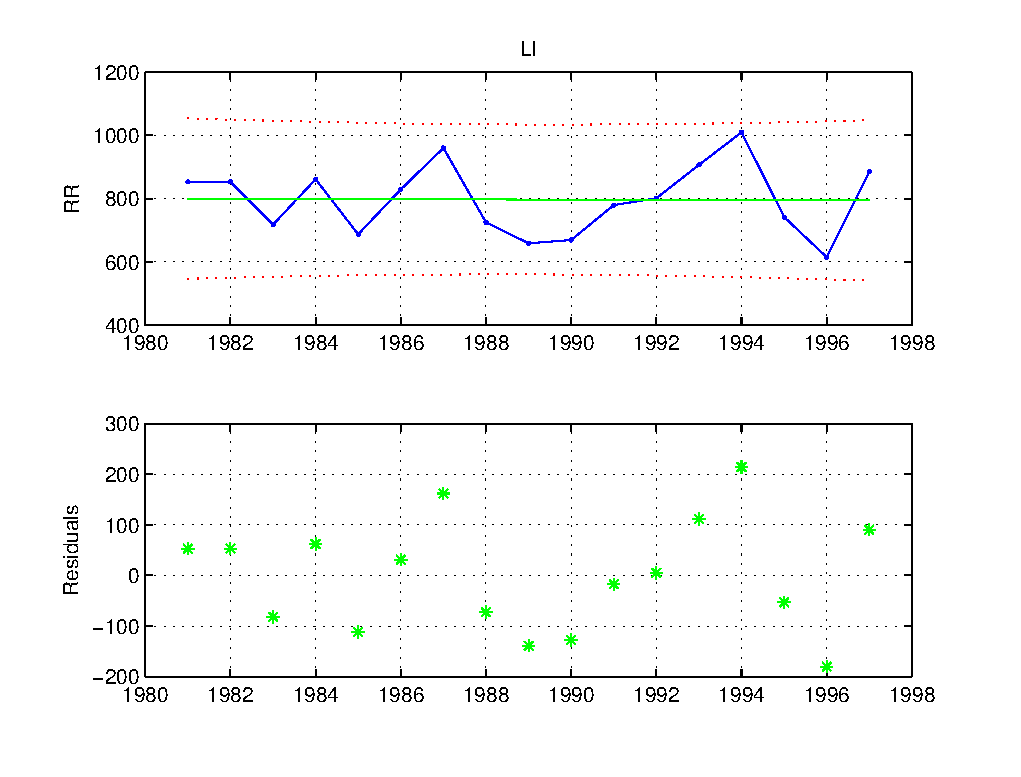
\includegraphics[width=0.33\textwidth]{./img/li_rr}}
  \subfloat[HPF]{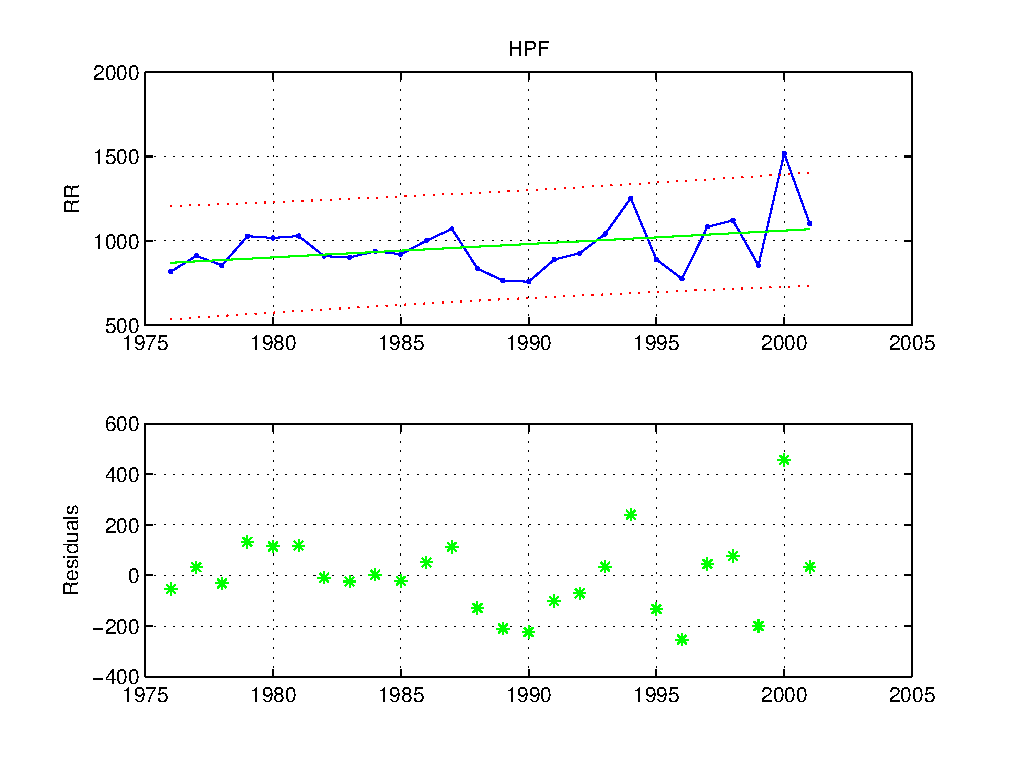
\includegraphics[width=0.33\textwidth]{./img/hpf_rr}}

  \subfloat[HD]{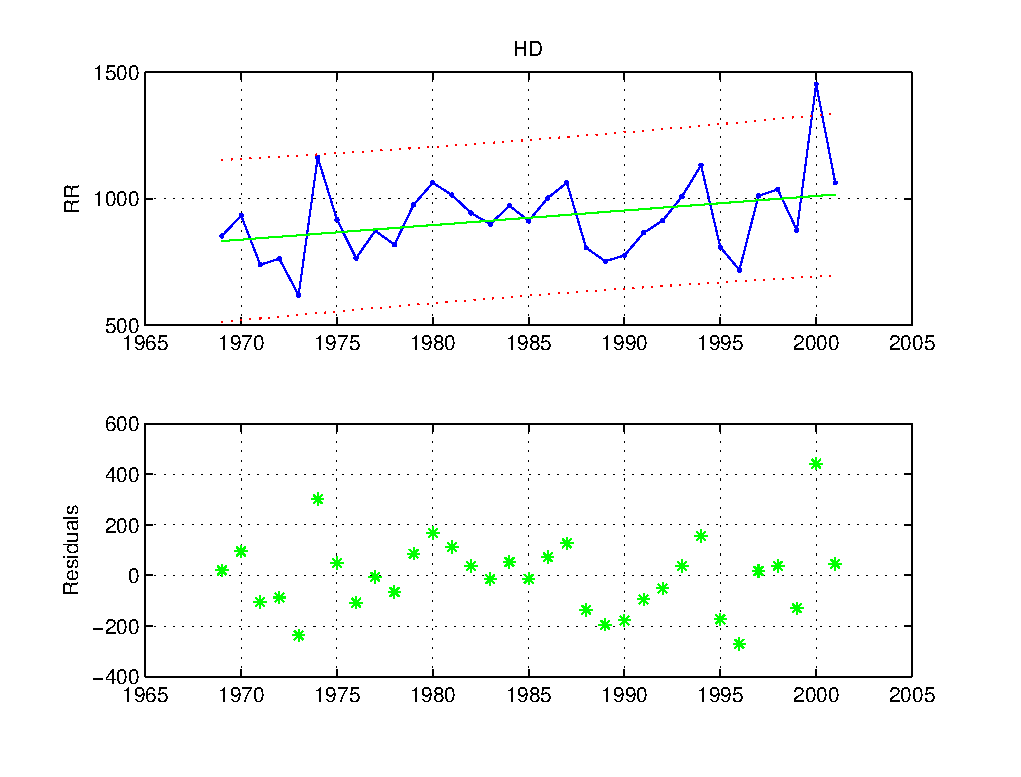
\includegraphics[width=0.33\textwidth]{./img/hd_rr}}
  \subfloat[FF]{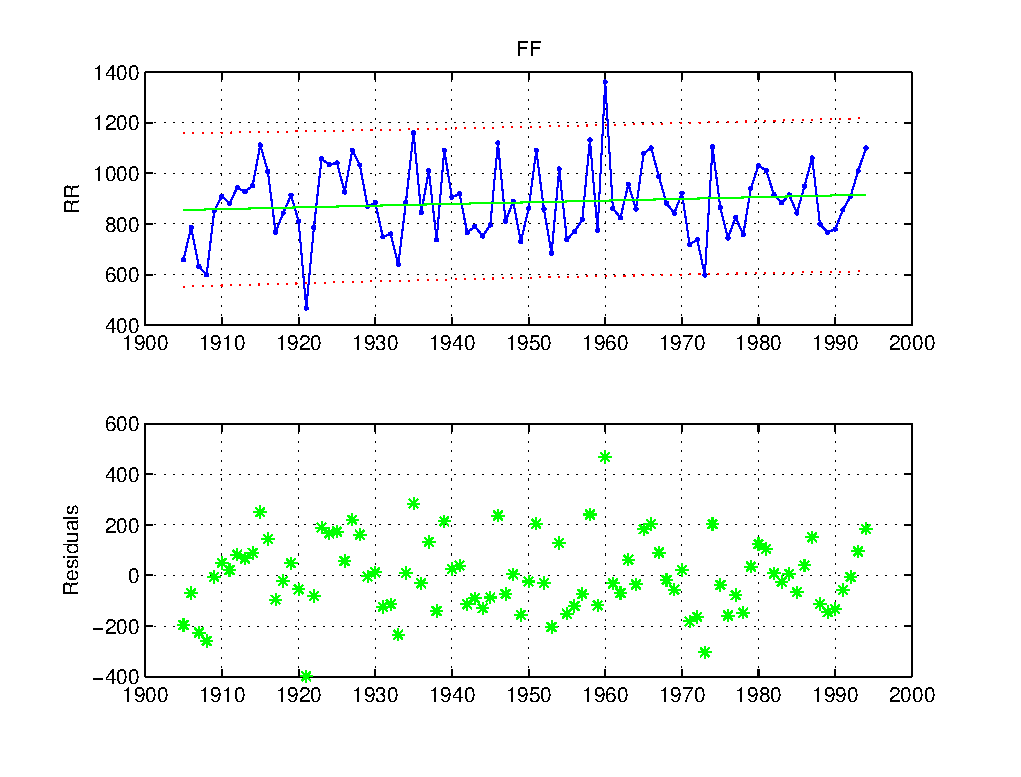
\includegraphics[width=0.33\textwidth]{./img/ff_rr}}
  \caption{Trends of annual rainfall amount (RR) at daily data stations}
  \label{fig:FF_annual_RR}
\end{figure}

\paragraph{Number of Wet Days (RR1)}
\label{sec:NumberOfRaindaysRR1}

The number of wet days per year decreased at PL and FF stations (M-K, $p<0.05$)
(Figure \ref{fig:FF_annual_RR1}). Although not all the stations showed
statistically significant annual trends, the ones with significant annual trend
in the number of wet days show downward trends in the number of wet days over
the data periods.
%A downward annual trend was also confirmed by Mann-Kendall test ($p<0.05$) for
%the same periods.

The month of March shows significant decreasing trends in the number of wet days
per month over 1980--1999. The month of July also shows decreasing trend in the
recent decade.

\begin{figure}[htbp]
  \centering
  \subfloat[DR]{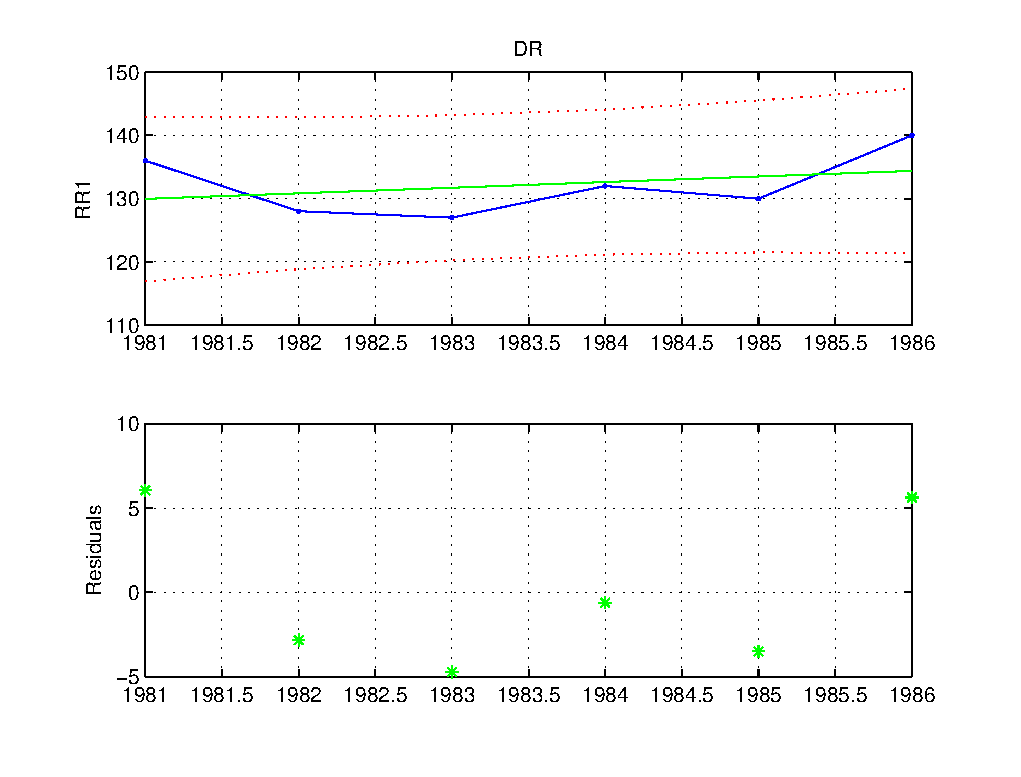
\includegraphics[width=0.33\textwidth]{./img/dr_rr1}}
  \subfloat[SO]{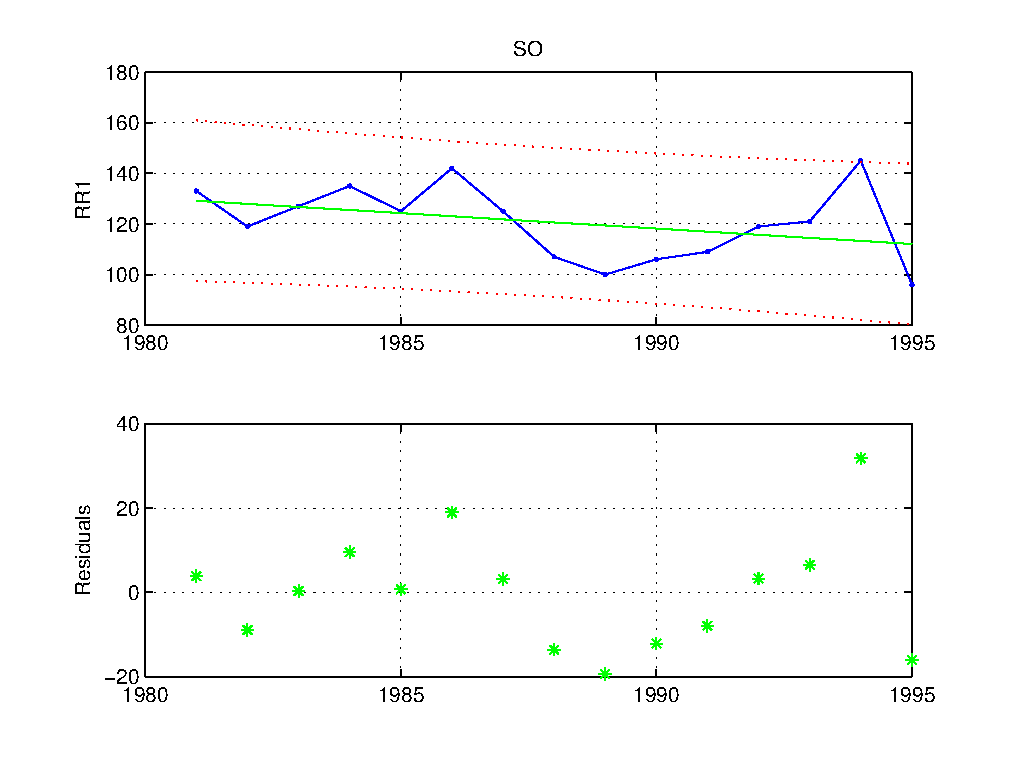
\includegraphics[width=0.33\textwidth]{./img/so_rr1}}
  \subfloat[PL]{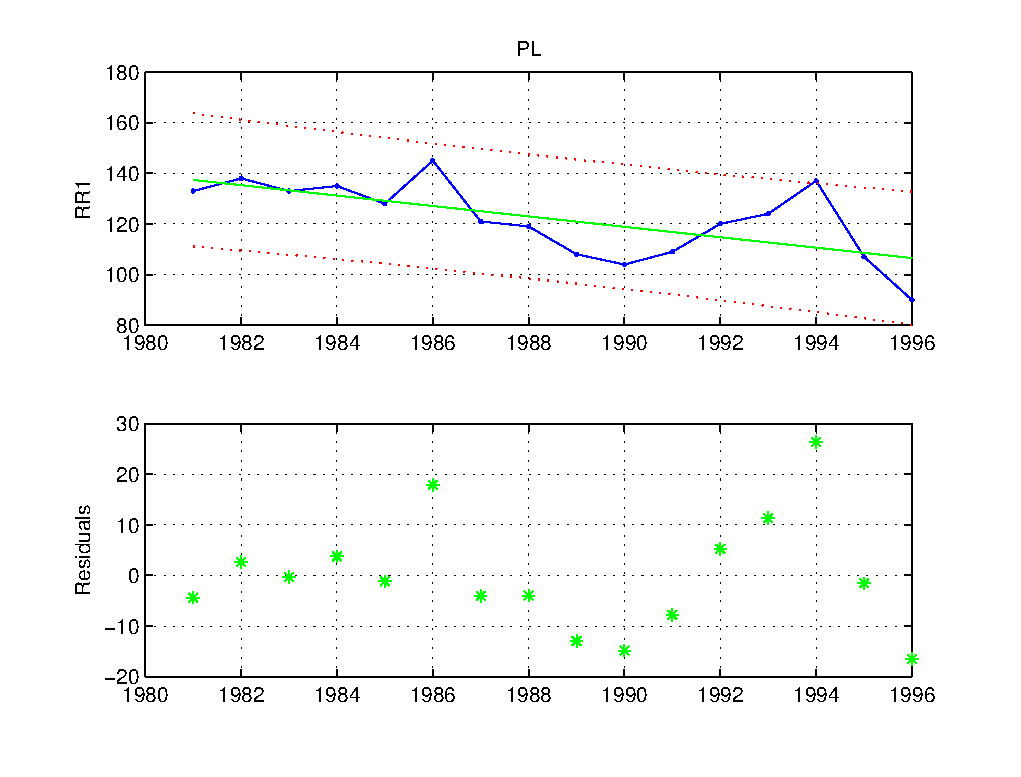
\includegraphics[width=0.33\textwidth]{./img/pl_rr1}}

  \subfloat[PB]{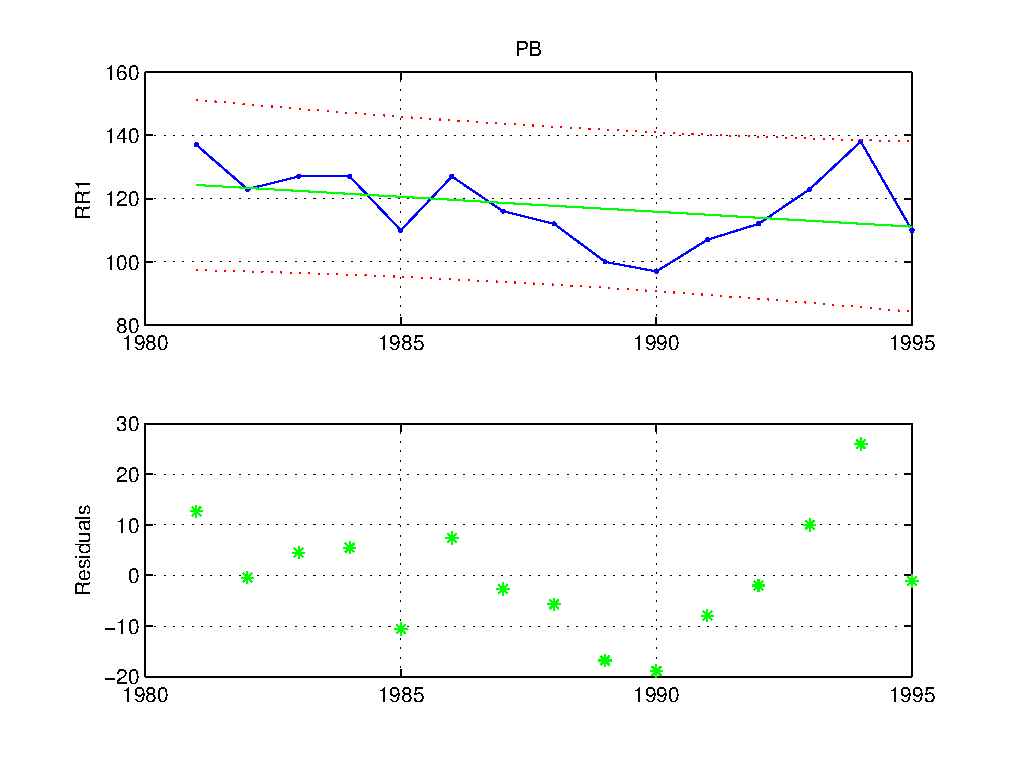
\includegraphics[width=0.33\textwidth]{./img/pb_rr1}}
  \subfloat[SDR]{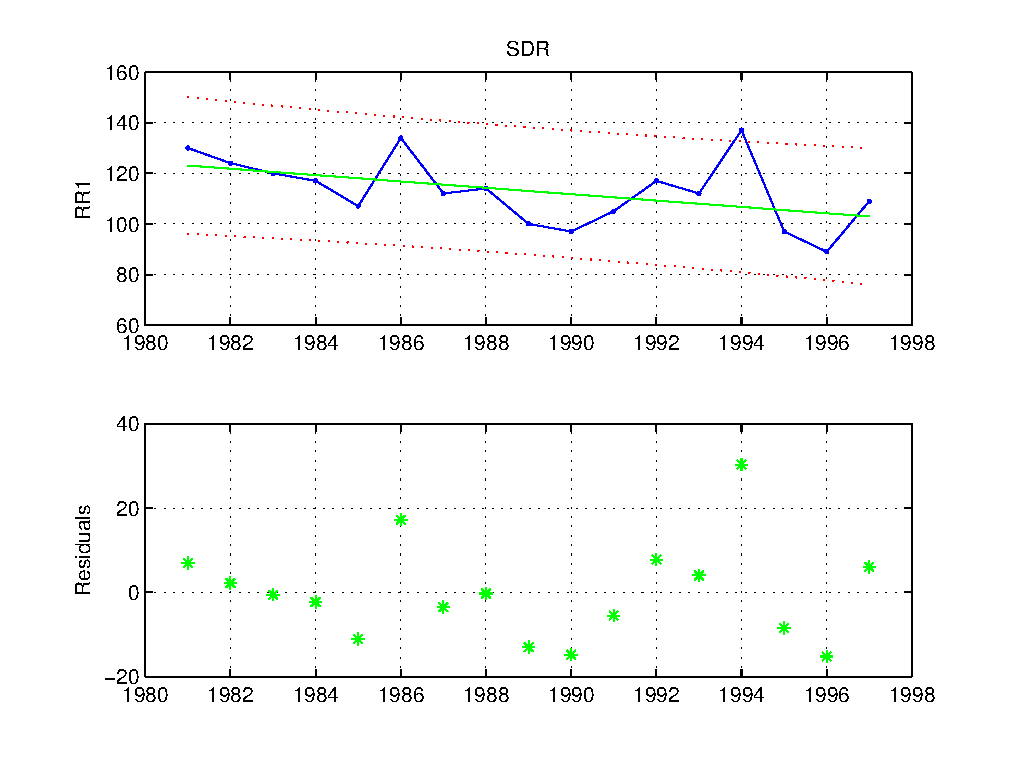
\includegraphics[width=0.33\textwidth]{./img/sdr_rr1}}
  \subfloat[EW]{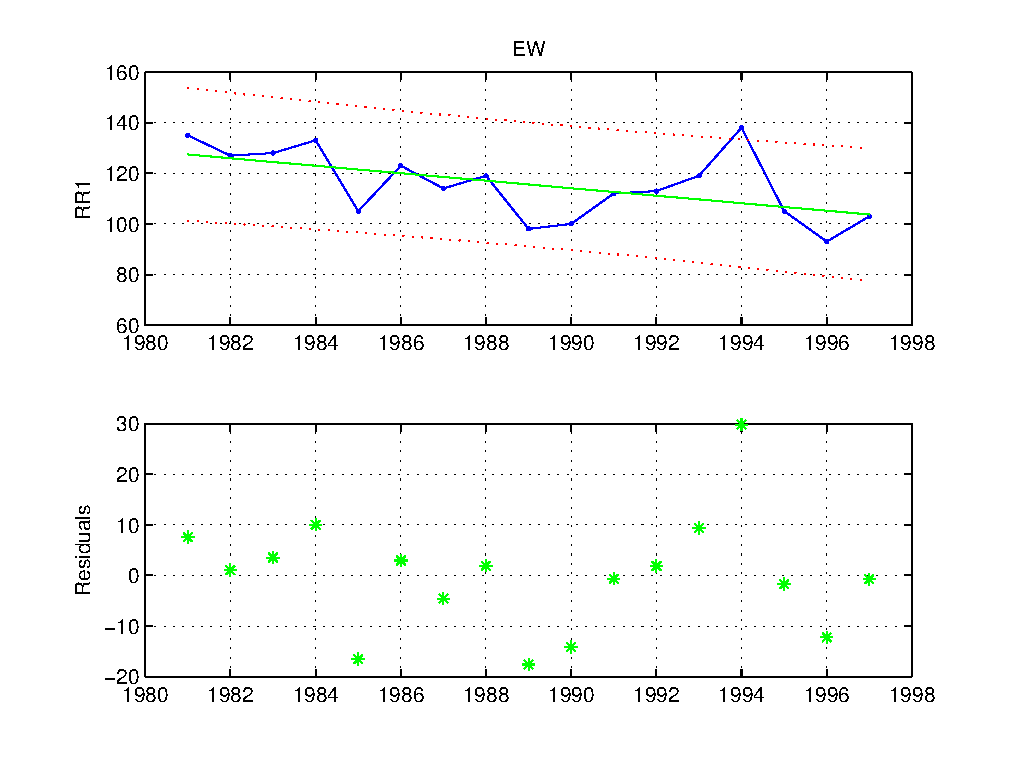
\includegraphics[width=0.33\textwidth]{./img/ew_rr1}}

  \subfloat[FT]{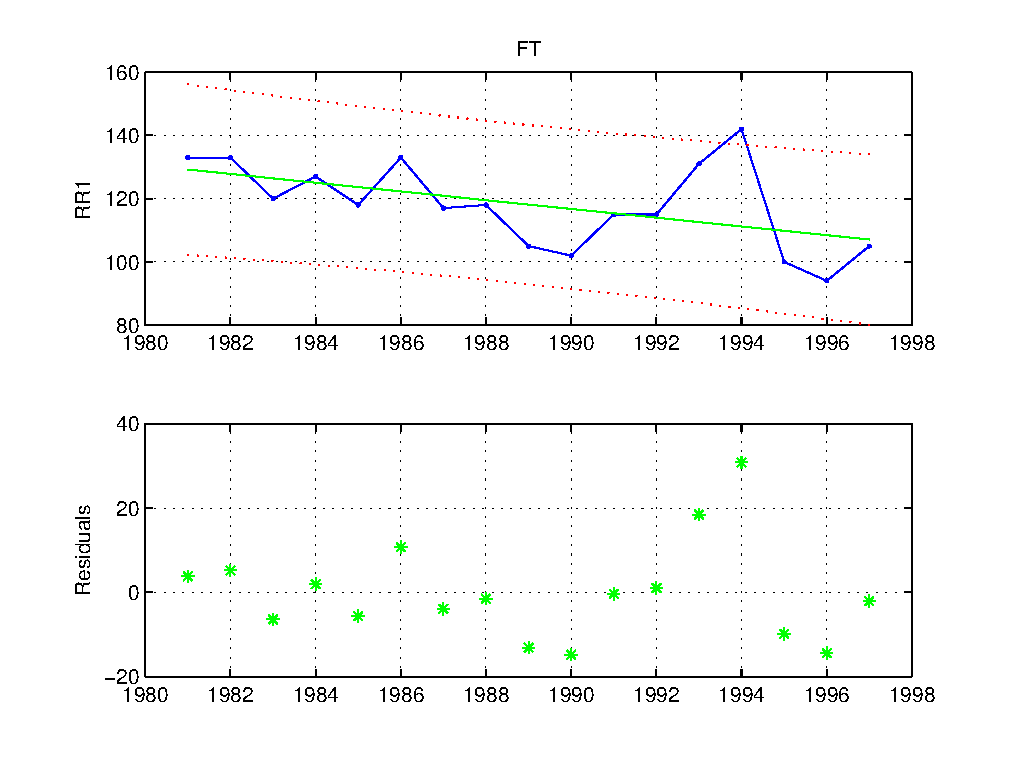
\includegraphics[width=0.33\textwidth]{./img/ft_rr1}}
  \subfloat[LI]{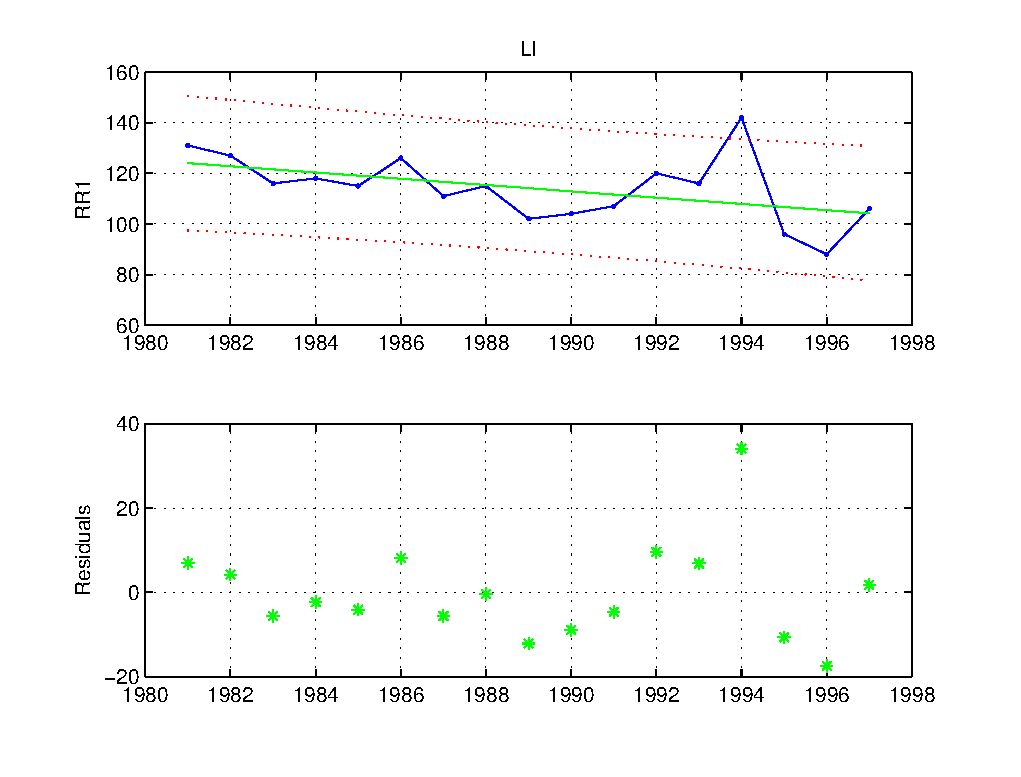
\includegraphics[width=0.33\textwidth]{./img/li_rr1}}
  \subfloat[HPF]{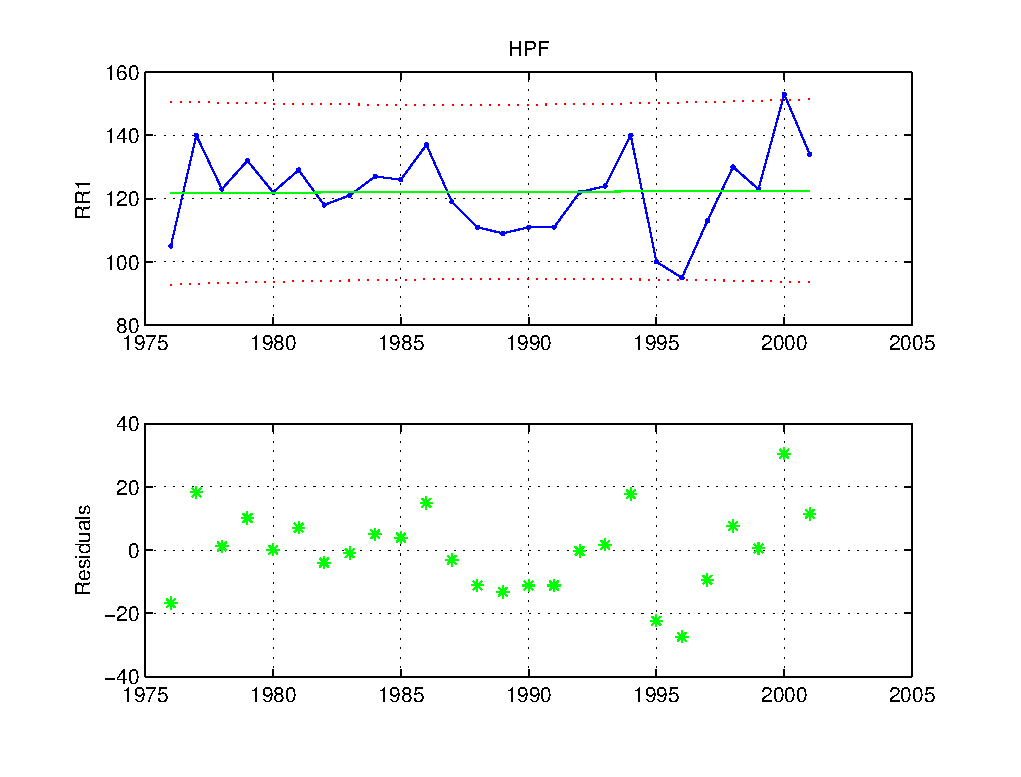
\includegraphics[width=0.33\textwidth]{./img/hpf_rr1}}

  \subfloat[HD]{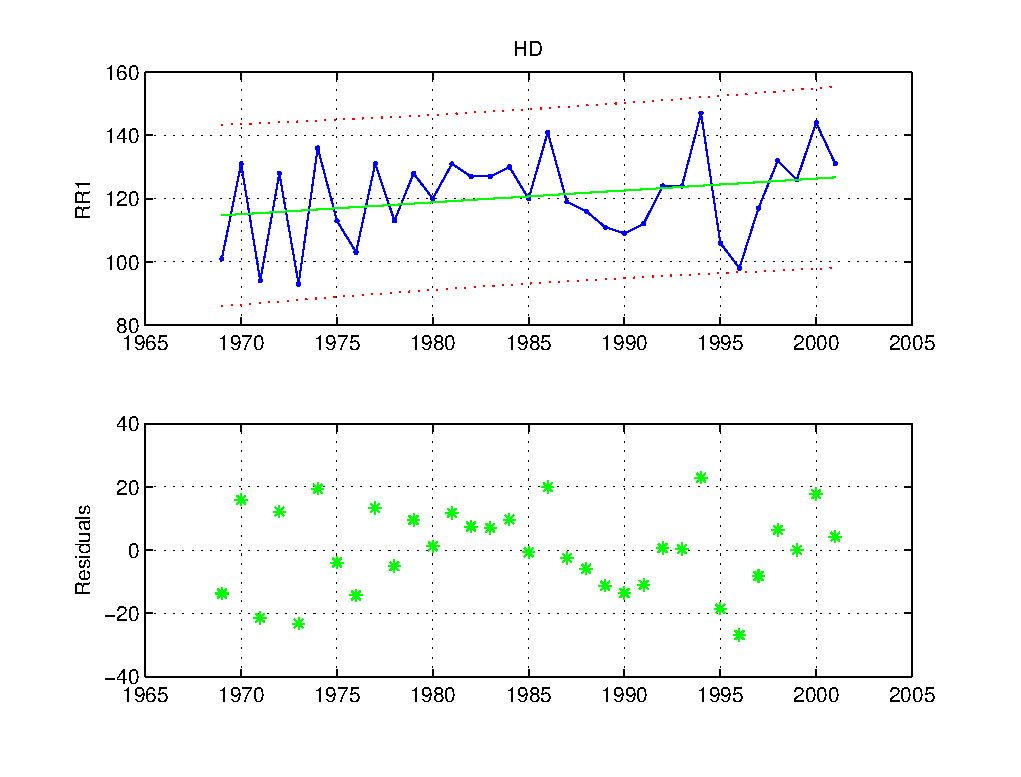
\includegraphics[width=0.33\textwidth]{./img/hd_rr1}}
  \subfloat[FF]{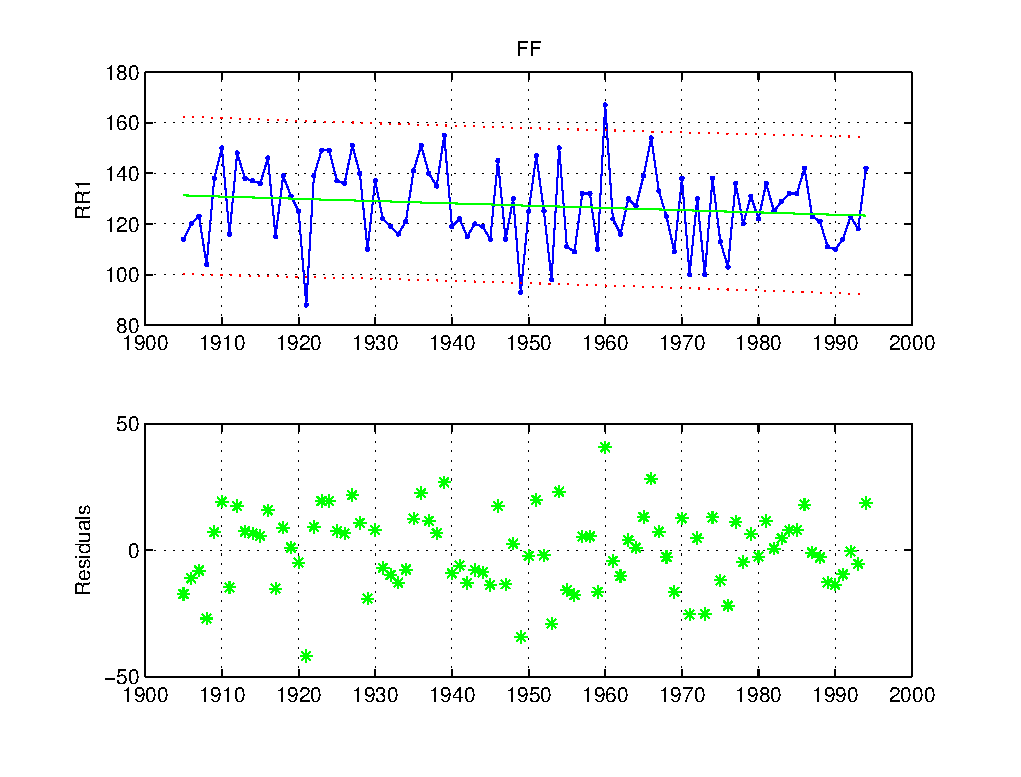
\includegraphics[width=0.33\textwidth]{./img/ff_rr1}}
  \caption{Trends of number of wetdays (RR1) at daily data stations}
  \label{fig:FF_annual_RR1}
\end{figure}

\paragraph{Simple Daily Intensity Index (SDII)}
\label{sec:SimpleDailyIntensityIndex}
As expected, PL \& FF again showed a significant annual trend in SDII. The rest
of the stations showed no significant results. FF station showed upward annual
trends in SDII throughout the data periods (Figure \ref{fig:FF_annual_SDII}).
All the cases with significant trends exhibited increasing trend of annual
SDII.

\begin{figure}[htbp]
  \centering
  \subfloat[DR]{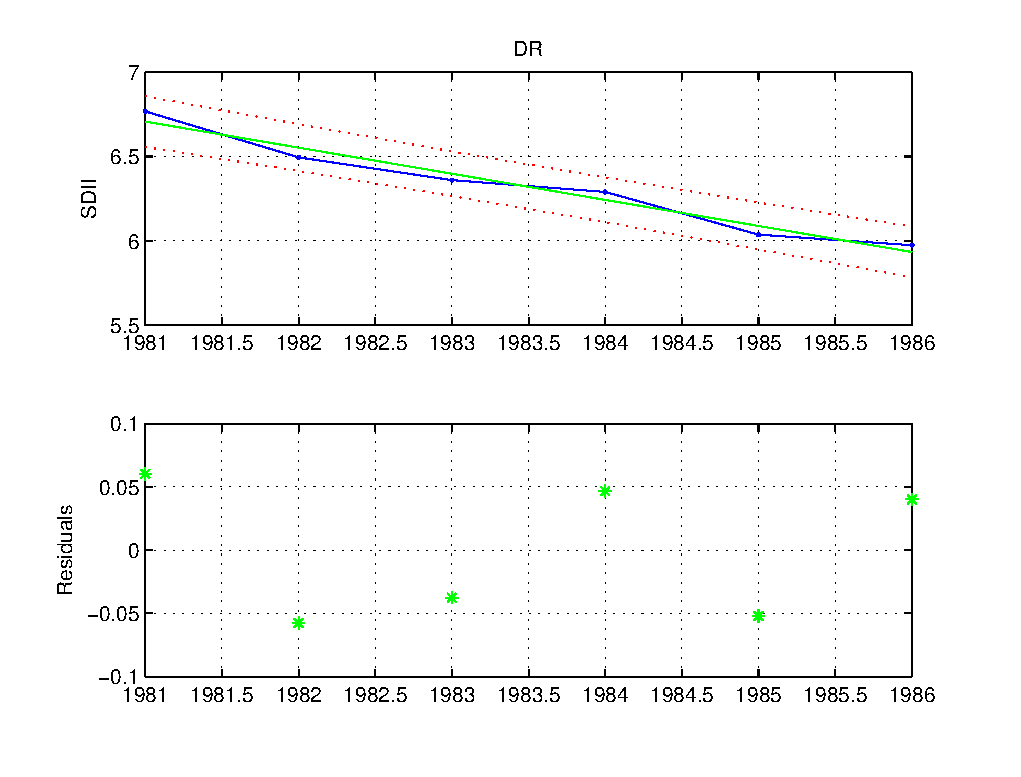
\includegraphics[width=0.33\textwidth]{./img/dr_sdii}}
  \subfloat[SO]{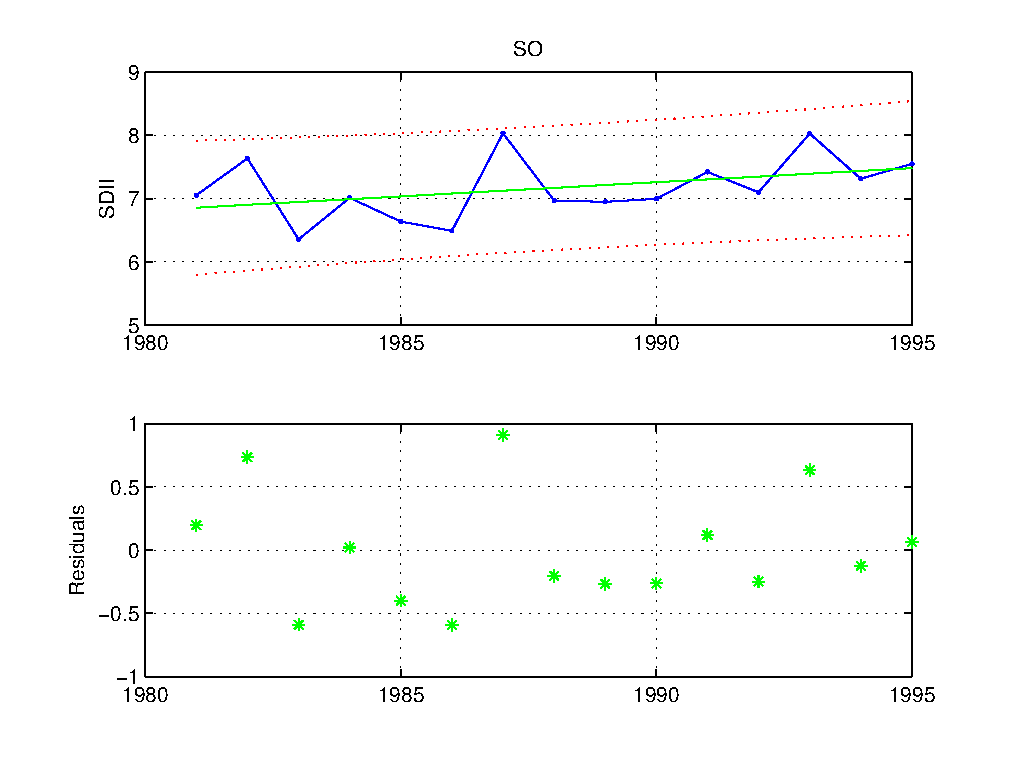
\includegraphics[width=0.33\textwidth]{./img/so_sdii}}
  \subfloat[PL]{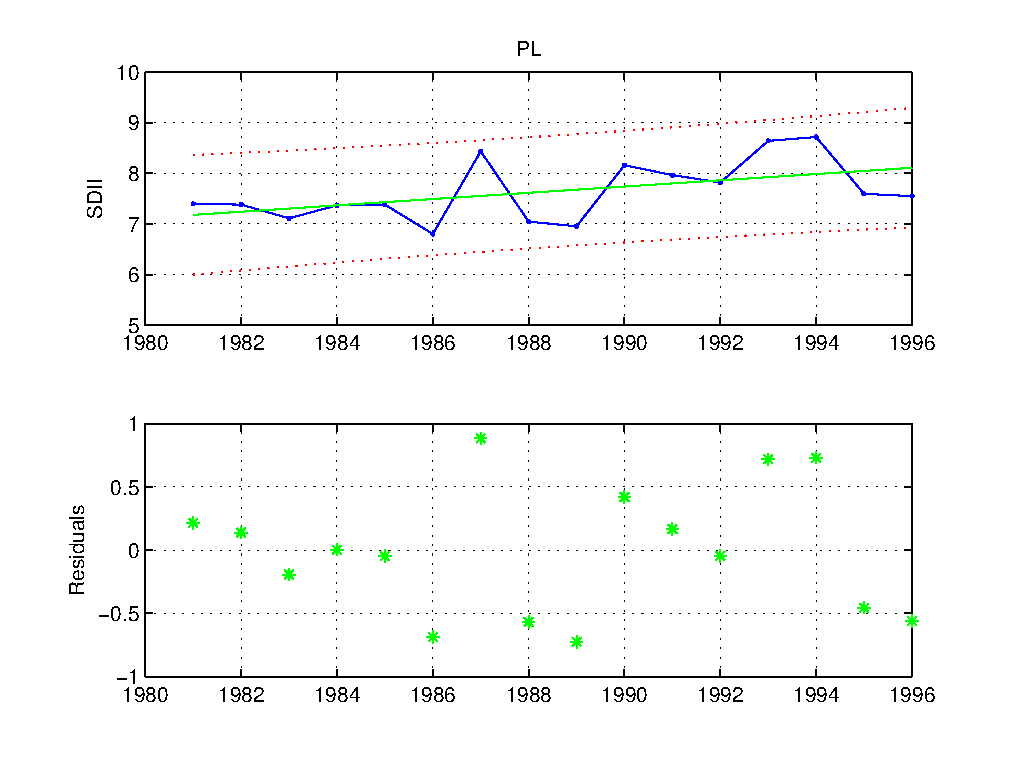
\includegraphics[width=0.33\textwidth]{./img/pl_sdii}}

  \subfloat[PB]{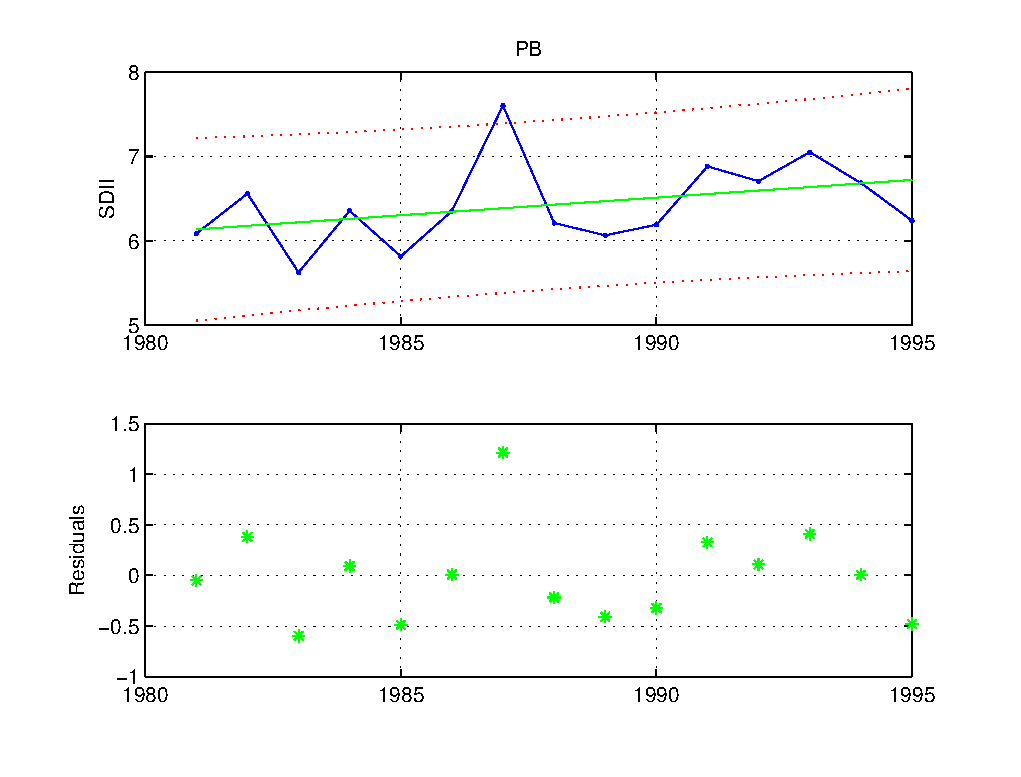
\includegraphics[width=0.33\textwidth]{./img/pb_sdii}}
  \subfloat[SDR]{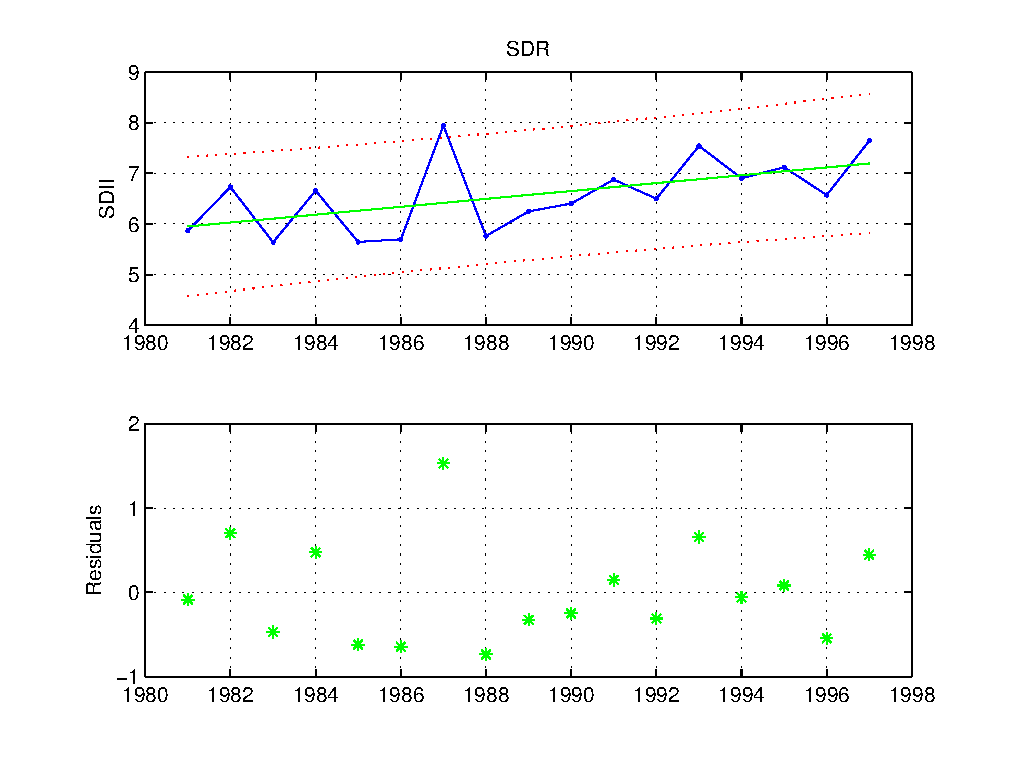
\includegraphics[width=0.33\textwidth]{./img/sdr_sdii}}
  \subfloat[EW]{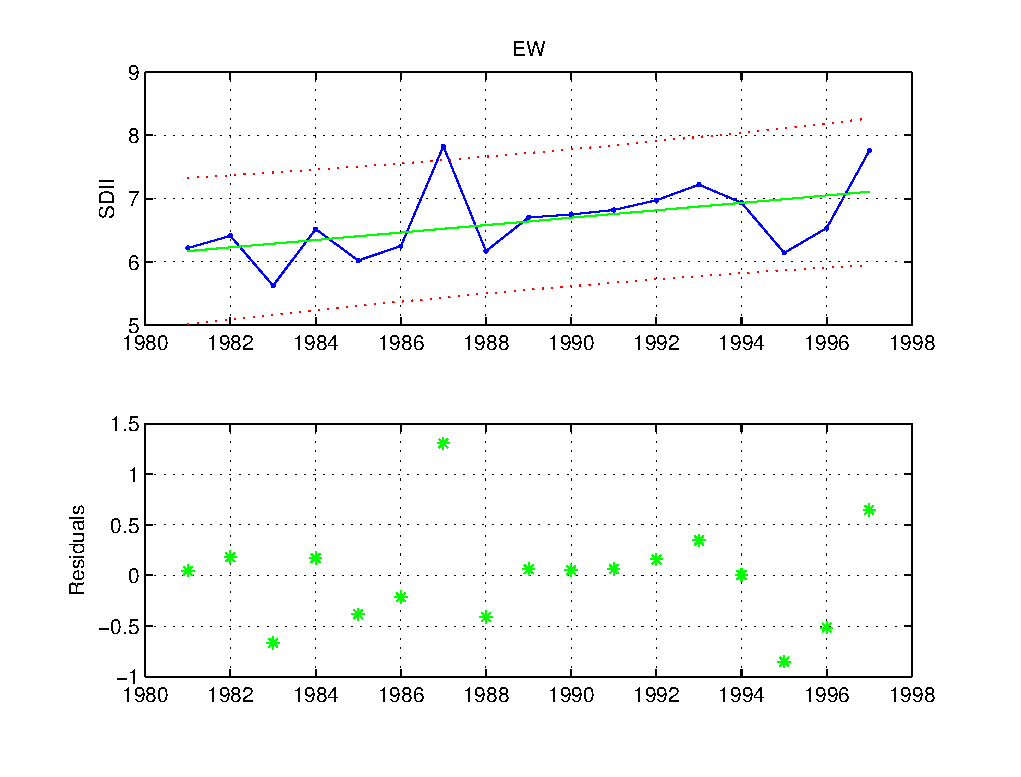
\includegraphics[width=0.33\textwidth]{./img/ew_sdii}}

  \subfloat[FT]{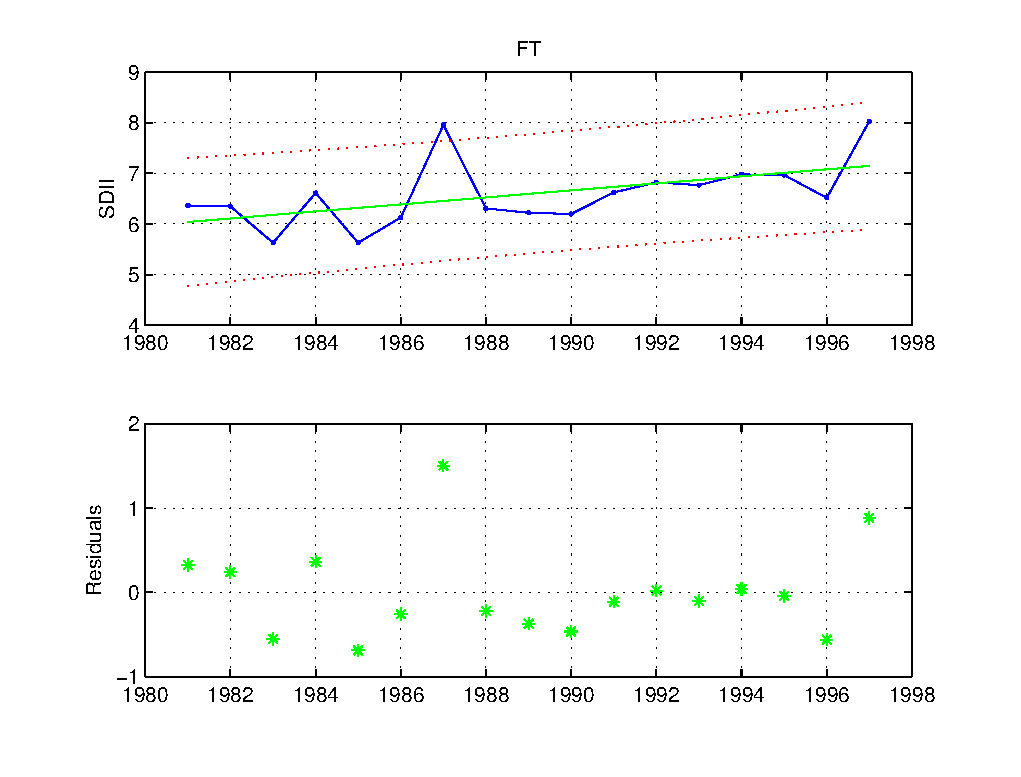
\includegraphics[width=0.33\textwidth]{./img/ft_sdii}}
  \subfloat[LI]{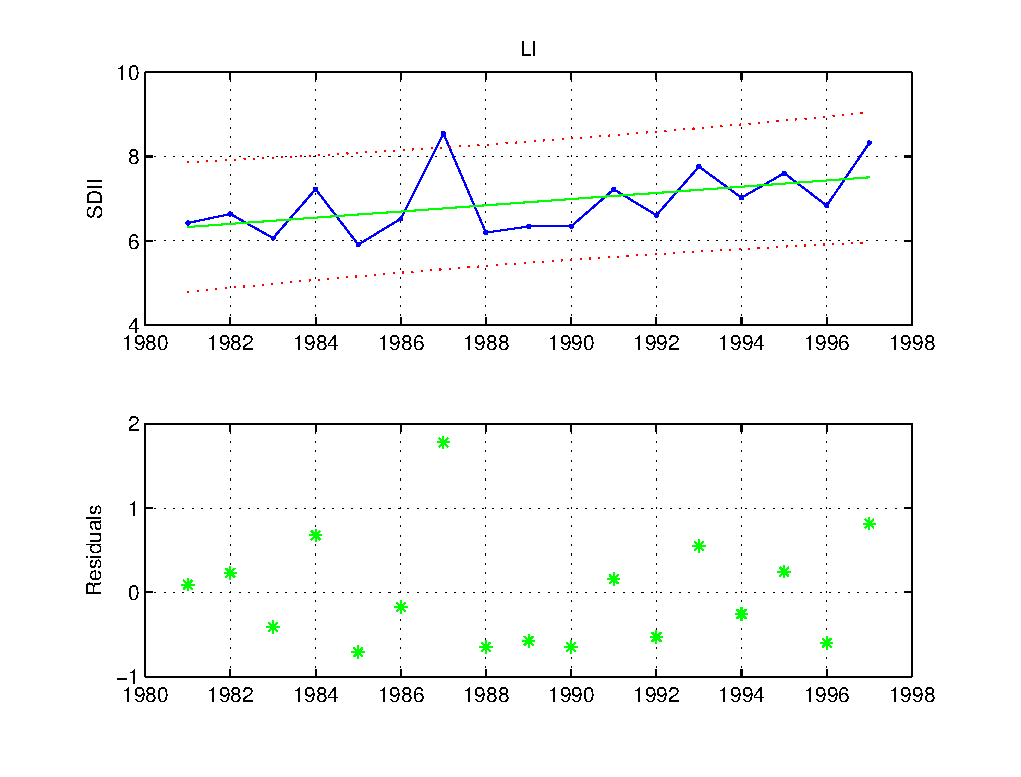
\includegraphics[width=0.33\textwidth]{./img/li_sdii}}
  \subfloat[HPF]{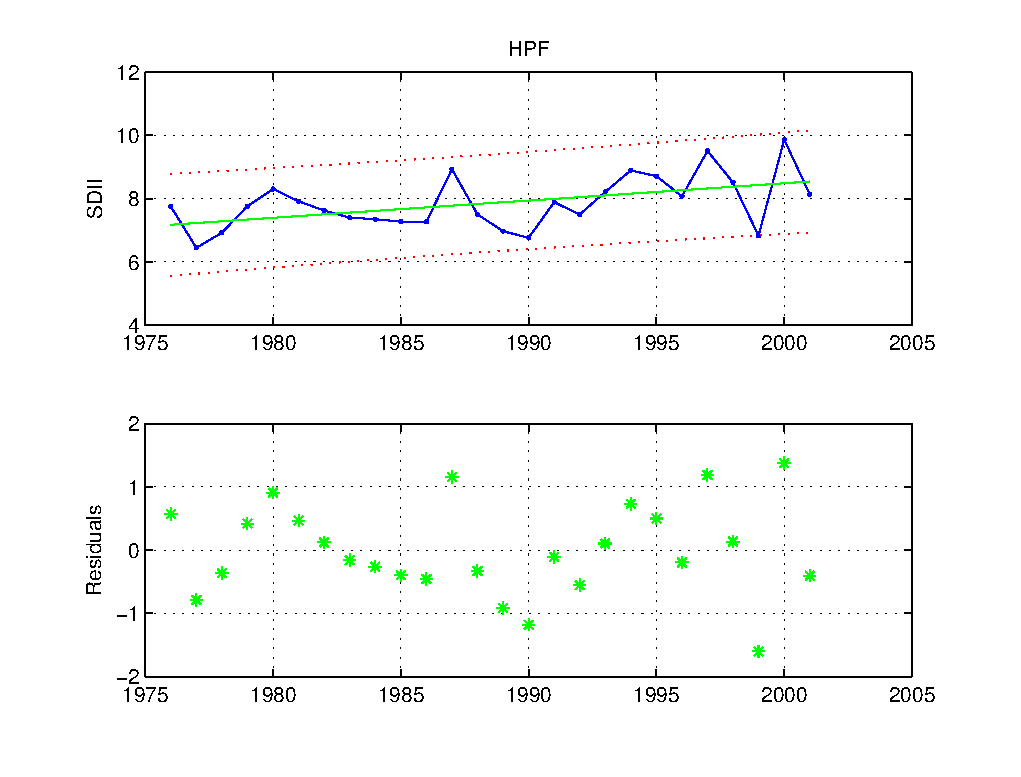
\includegraphics[width=0.33\textwidth]{./img/hpf_sdii}}

  \subfloat[HD]{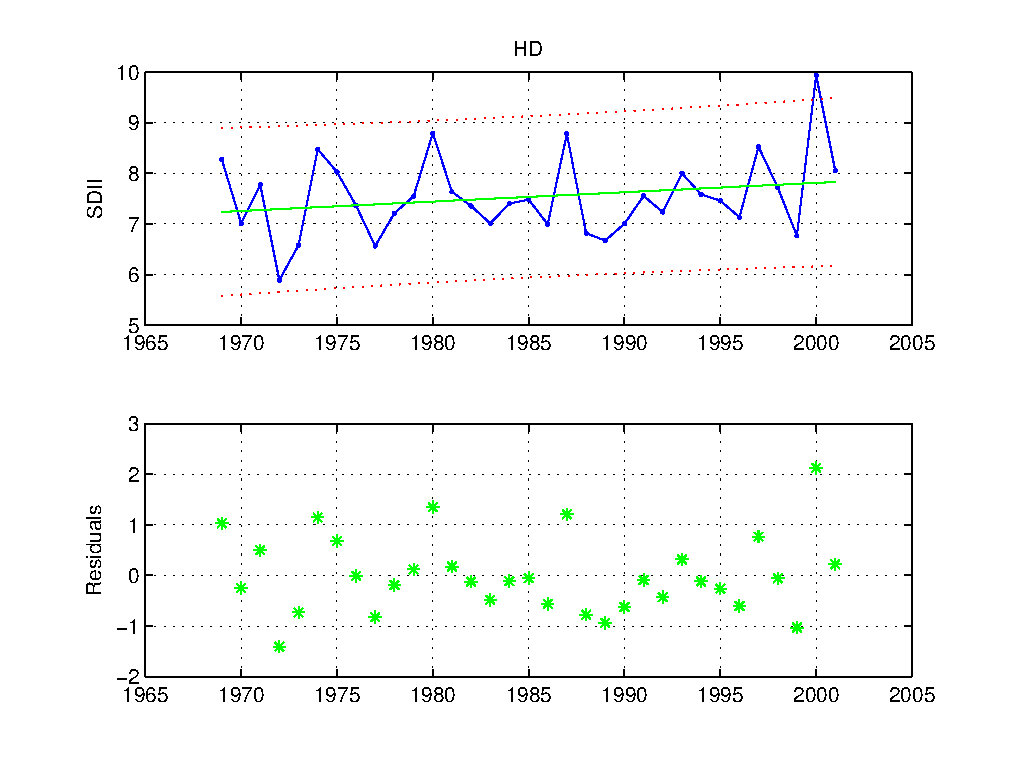
\includegraphics[width=0.33\textwidth]{./img/hd_sdii}}
  \subfloat[FF]{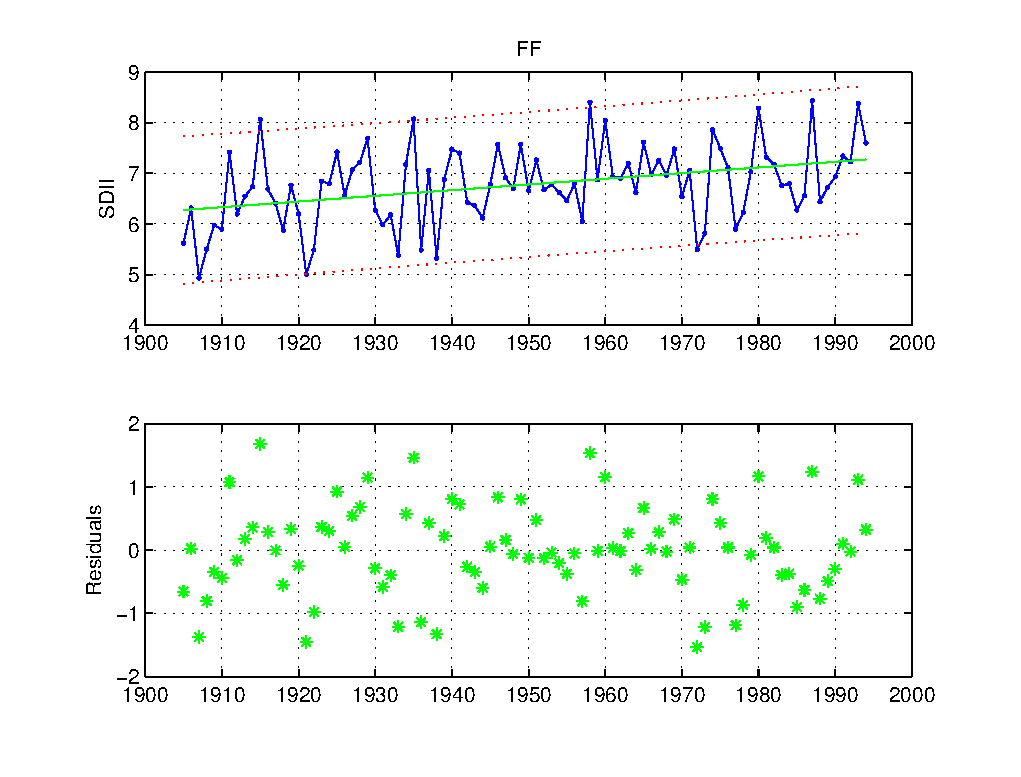
\includegraphics[width=0.33\textwidth]{./img/ff_sdii}}
  \caption{Trend of annual simple daily intensity index (SDII) at daily
data stations}
  \label{fig:FF_annual_SDII}
\end{figure}

\paragraph{Number of Days with Precipitation Amount $\geq$ 10 mm (R10mm)}
\label{sec:R10}
Annual trends of number of wet days with precipitation amount greater than 10 mm
(R10mm) from the studied stations are at variance. Only Falmer Farm Station
shows a statistically significant upwards trend for the 1971--1996 period (M-K,
$p<0.05$) (Figure \ref{fig:FF_annual_R10mm}). PL ($p < 0.05$) and FF ($p \ll
0.05$) show a statistically significant increasing trend in the annual ratio of
number of wet days with rainfall amount greater than 10 mm (Figure
\ref{fig:FF_annual_R10-b}).

\begin{figure}[htbp]
  \centering
  \subfloat[DR]{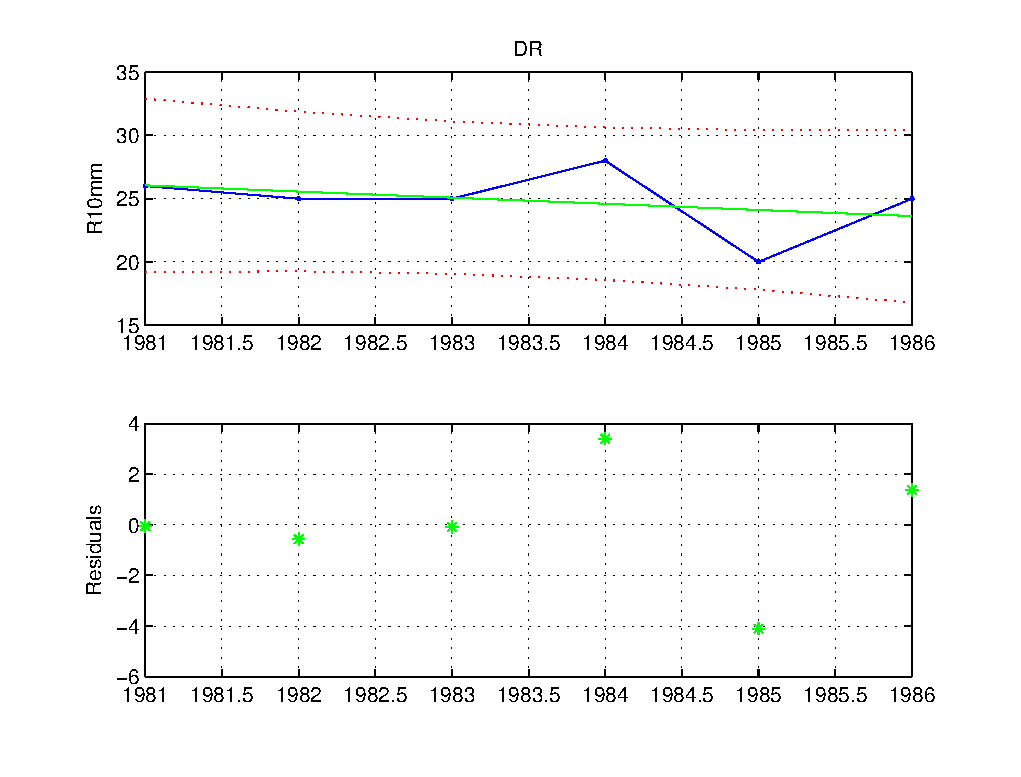
\includegraphics[width=0.33\textwidth]{./img/dr_r10mm}}
  \subfloat[SO]{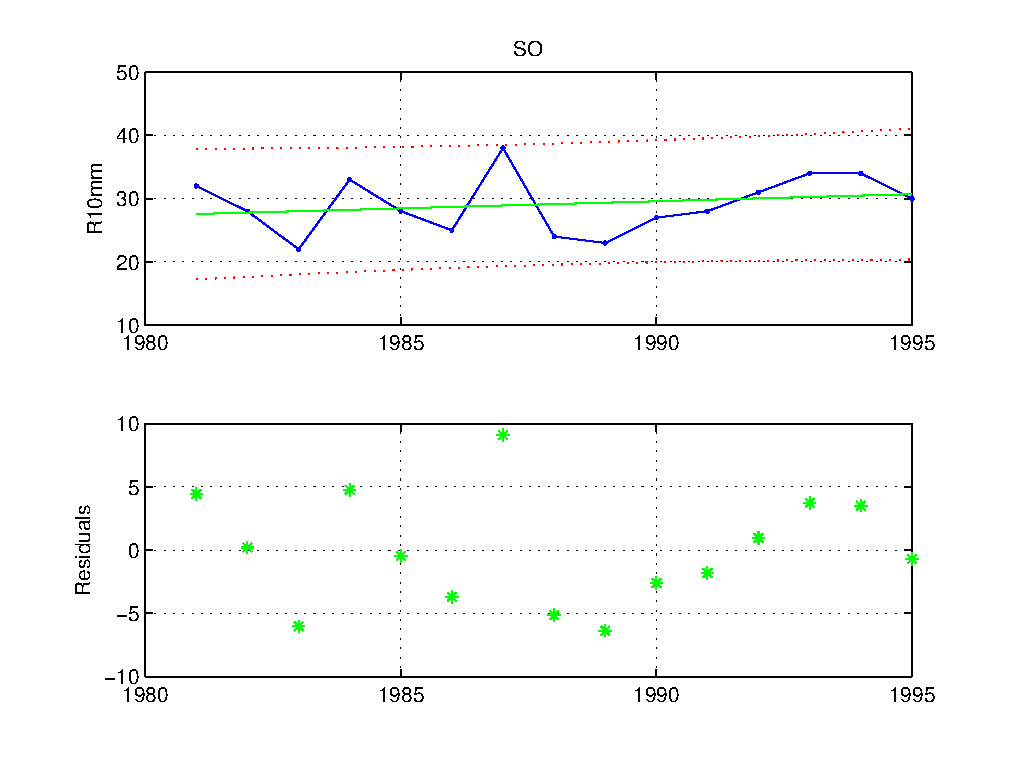
\includegraphics[width=0.33\textwidth]{./img/so_r10mm}}
  \subfloat[PL]{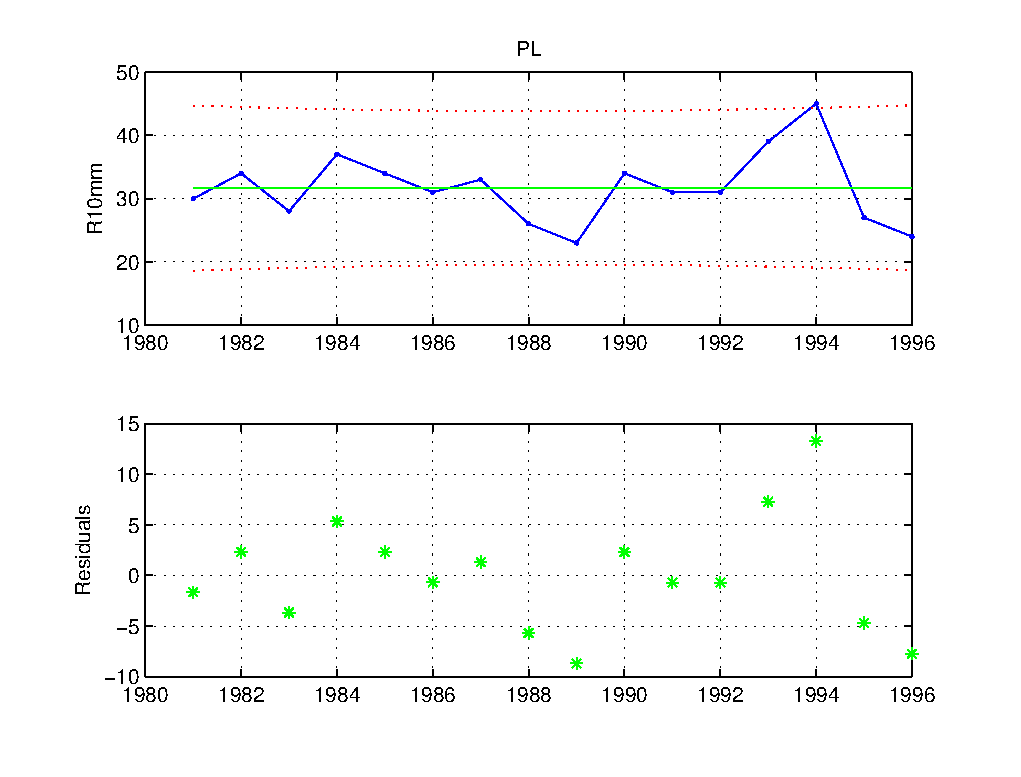
\includegraphics[width=0.33\textwidth]{./img/pl_r10mm}}

  \subfloat[PB]{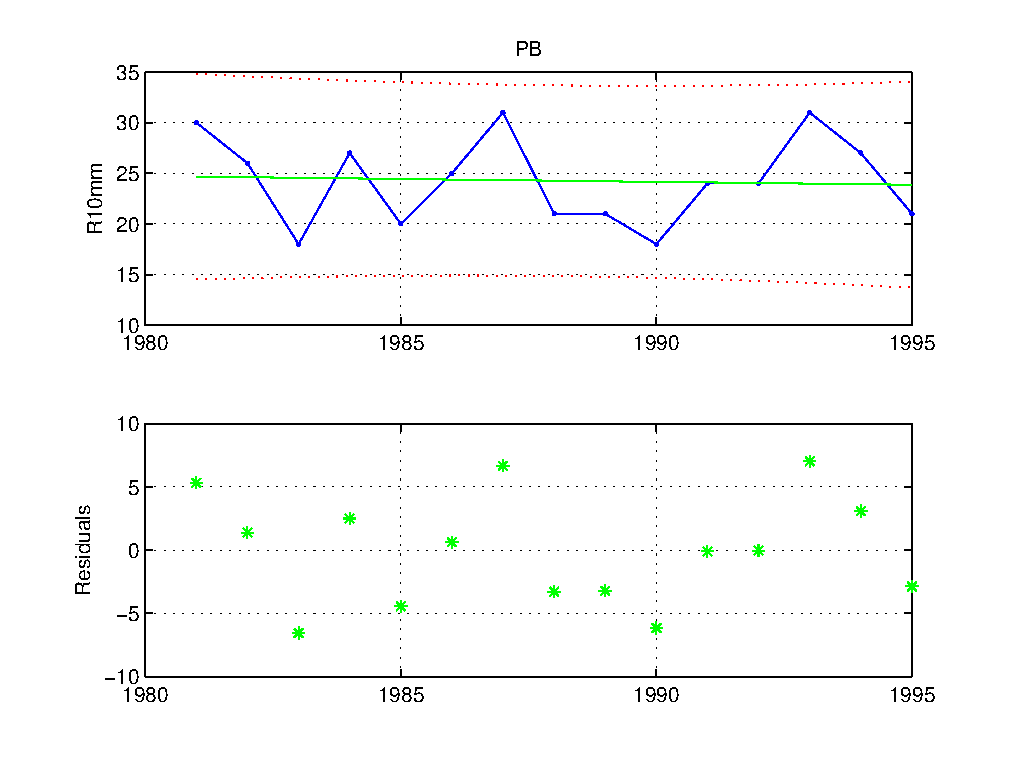
\includegraphics[width=0.33\textwidth]{./img/pb_r10mm}}
  \subfloat[SDR]{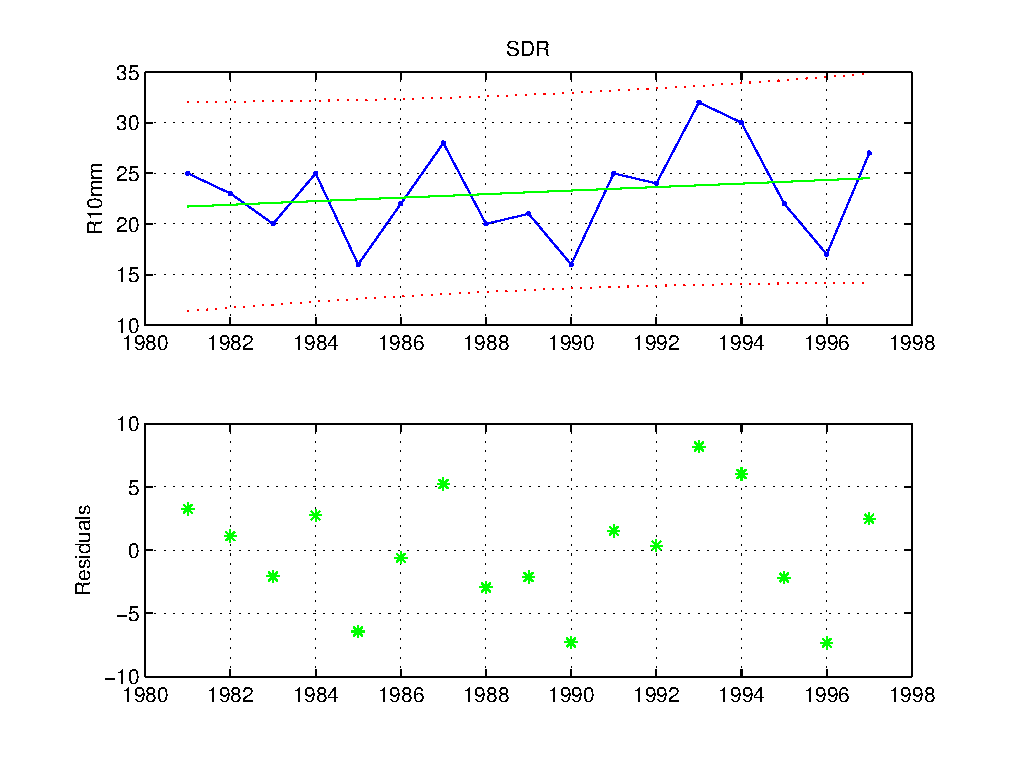
\includegraphics[width=0.33\textwidth]{./img/sdr_r10mm}}
  \subfloat[EW]{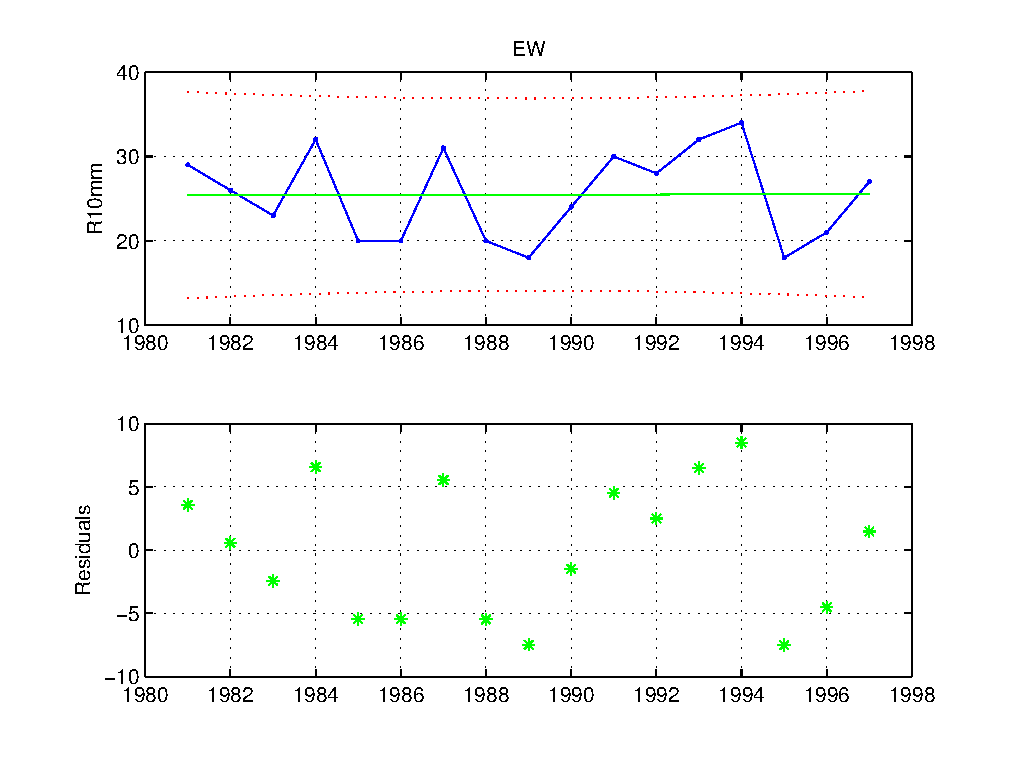
\includegraphics[width=0.33\textwidth]{./img/ew_r10mm}}

  \subfloat[FT]{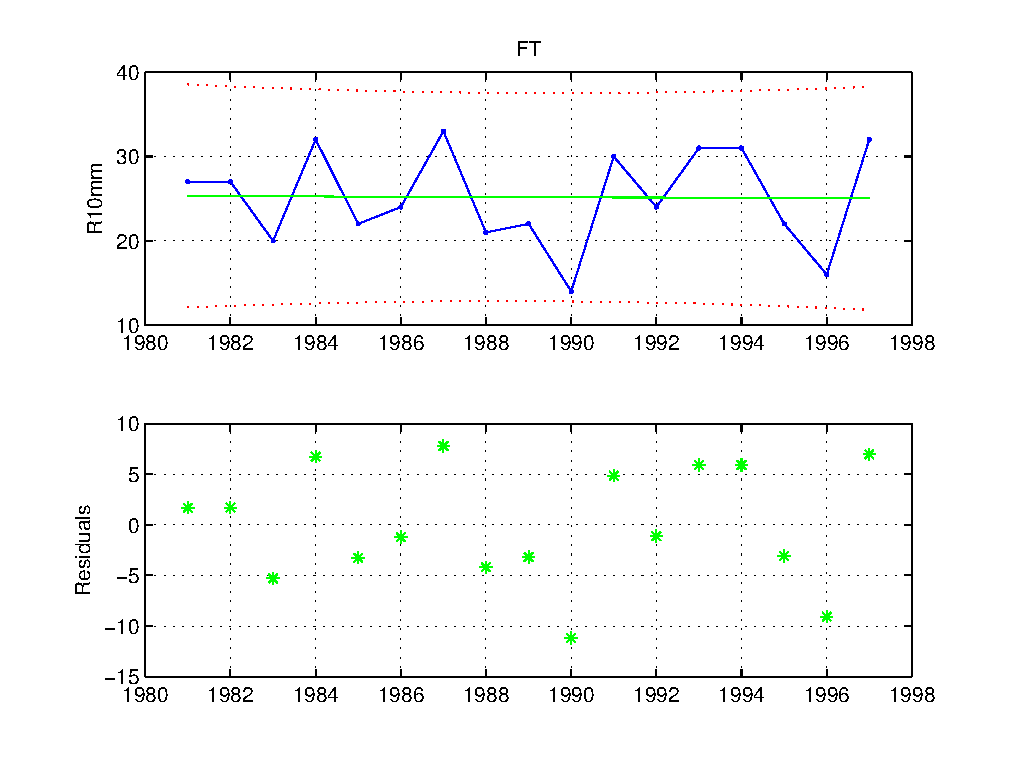
\includegraphics[width=0.33\textwidth]{./img/ft_r10mm}}
  \subfloat[LI]{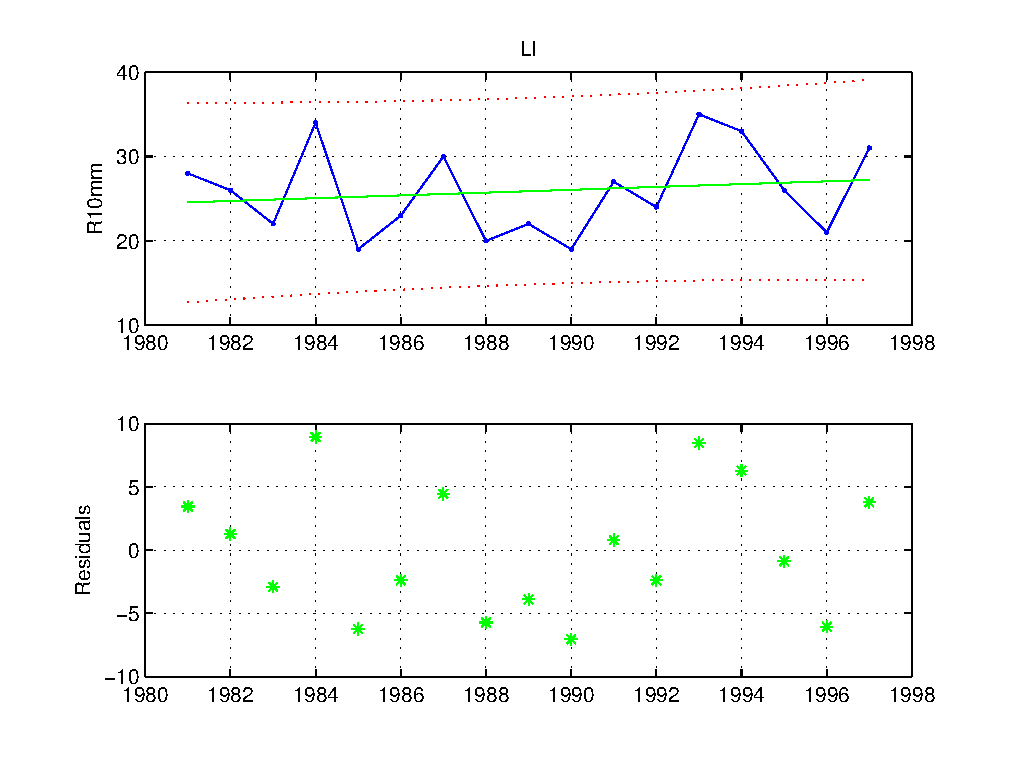
\includegraphics[width=0.33\textwidth]{./img/li_r10mm}}
  \subfloat[HPF]{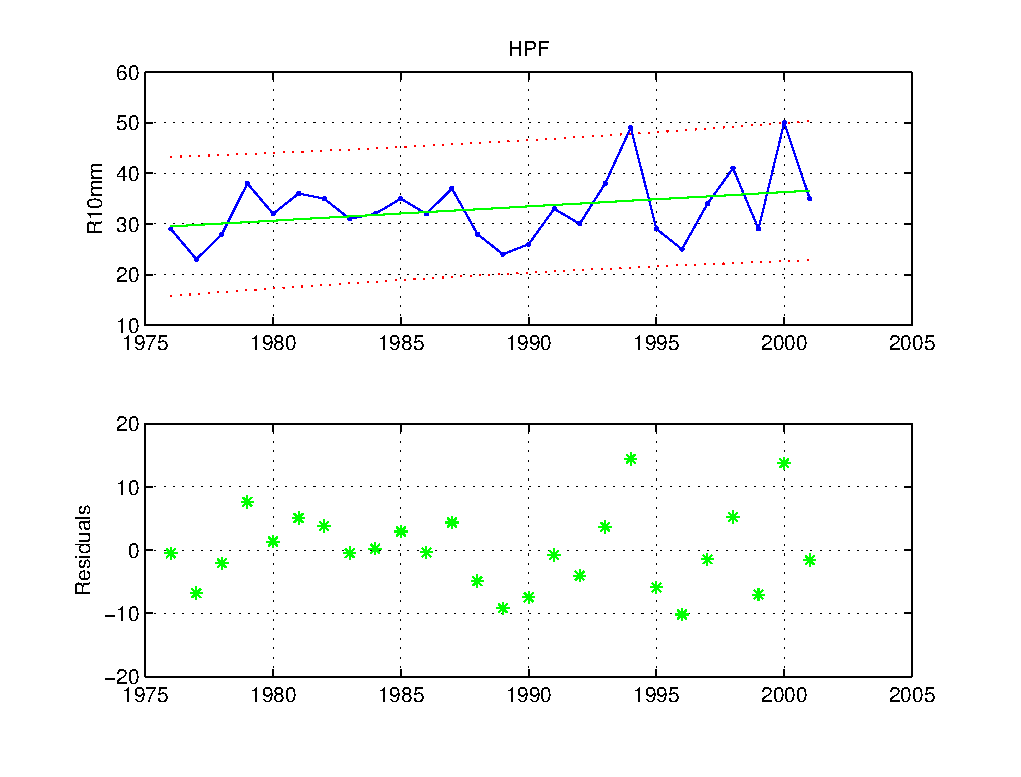
\includegraphics[width=0.33\textwidth]{./img/hpf_r10mm}}

  \subfloat[HD]{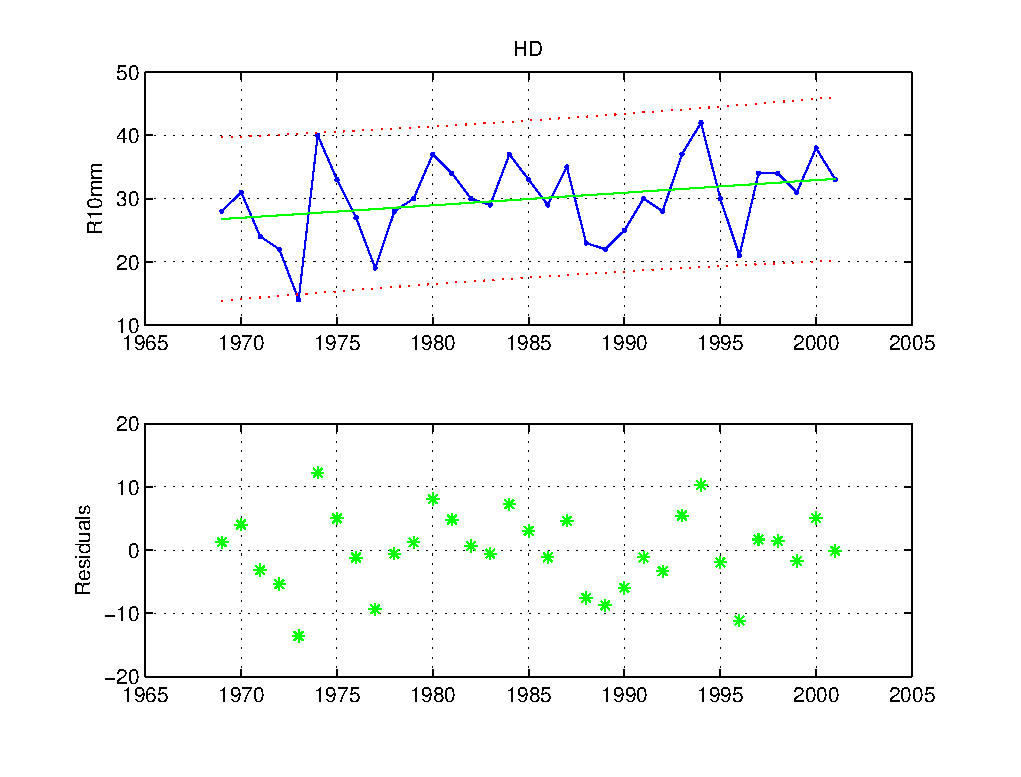
\includegraphics[width=0.33\textwidth]{./img/hd_r10mm}}
  \subfloat[FF]{\includegraphics[width=0.33\textwidth]{./img/ff_r10mm}
\label{fig:FF_annual_R10-a}}
  \caption{Annual number of wet days with rainfall amount $\geq$ 10 mm at
daily data stations}
  \label{fig:FF_annual_R10mm}
\end{figure}

\begin{figure}[htbp]
  \centering
  \subfloat[DR]{\includegraphics[width=0.33\textwidth]{./img/dr_r10p}}
  \subfloat[SO]{\includegraphics[width=0.33\textwidth]{./img/so_r10p}}
  \subfloat[PL]{\includegraphics[width=0.33\textwidth]{./img/pl_r10p}}

  \subfloat[PB]{\includegraphics[width=0.33\textwidth]{./img/pb_r10p}}
  \subfloat[SDR]{\includegraphics[width=0.33\textwidth]{./img/sdr_r10p}}
  \subfloat[EW]{\includegraphics[width=0.33\textwidth]{./img/ew_r10p}}

  \subfloat[FT]{\includegraphics[width=0.33\textwidth]{./img/ft_r10p}}
  \subfloat[LI]{\includegraphics[width=0.33\textwidth]{./img/li_r10p}}
  \subfloat[HPF]{\includegraphics[width=0.33\textwidth]{./img/hpf_r10p}}

  \subfloat[HD]{\includegraphics[width=0.33\textwidth]{./img/hd_r10p}}
  \subfloat[FF]{\includegraphics[width=0.33\textwidth]{./img/ff_r10p}
\label{fig:FF_annual_R10-b}}
  \caption{Annual \% of wet days with rainfall amount $\geq$ 10 mm at
daily data stations}
  \label{fig:FF_annual_R10p}
\end{figure}

\paragraph{Number of Days with Precipitation Amount $\geq$ 20 mm (R20mm)}
\label{sec:R20}
No station shows a significant trend in the annual number of wet days with
rainfall greater than 20 mm. A trend in the annual ratio of number of wet days
with rainfall amount over 20 mm was not detectable as well (Figure
\ref{fig:FF_annual_R20mm}).

\begin{figure}[htbp]
  \centering
  \subfloat[DR]{\includegraphics[width=0.33\textwidth]{./img/dr_r20mm}}
  \subfloat[SO]{\includegraphics[width=0.33\textwidth]{./img/so_r20mm}}
  \subfloat[PL]{\includegraphics[width=0.33\textwidth]{./img/pl_r20mm}}

  \subfloat[PB]{\includegraphics[width=0.33\textwidth]{./img/pb_r20mm}}
  \subfloat[SDR]{\includegraphics[width=0.33\textwidth]{./img/sdr_r20mm}}
  \subfloat[EW]{\includegraphics[width=0.33\textwidth]{./img/ew_r20mm}}

  \subfloat[FT]{\includegraphics[width=0.33\textwidth]{./img/ft_r20mm}}
  \subfloat[LI]{\includegraphics[width=0.33\textwidth]{./img/li_r20mm}}
  \subfloat[HPF]{\includegraphics[width=0.33\textwidth]{./img/hpf_r20mm}}

  \subfloat[HD]{\includegraphics[width=0.33\textwidth]{./img/hd_r20mm}}
  \subfloat[FF]{\includegraphics[width=0.33\textwidth]{./img/ff_r20mm}
\label{fig:FF_annual_R20-a}}
  \caption{Annual number of wet days with rainfall amount $\geq$ 20 mm at
daily data stations}
  \label{fig:FF_annual_R20mm}
\end{figure}

\begin{figure}[htbp]
  \centering
  \subfloat[DR]{\includegraphics[width=0.33\textwidth]{./img/dr_r20p}}
  \subfloat[SO]{\includegraphics[width=0.33\textwidth]{./img/so_r20p}}
  \subfloat[PL]{\includegraphics[width=0.33\textwidth]{./img/pl_r20p}}

  \subfloat[PB]{\includegraphics[width=0.33\textwidth]{./img/pb_r20p}}
  \subfloat[SDR]{\includegraphics[width=0.33\textwidth]{./img/sdr_r20p}}
  \subfloat[EW]{\includegraphics[width=0.33\textwidth]{./img/ew_r20p}}

  \subfloat[FT]{\includegraphics[width=0.33\textwidth]{./img/ft_r20p}}
  \subfloat[LI]{\includegraphics[width=0.33\textwidth]{./img/li_r20p}}
  \subfloat[HPF]{\includegraphics[width=0.33\textwidth]{./img/hpf_r20p}}

  \subfloat[HD]{\includegraphics[width=0.33\textwidth]{./img/hd_r20p}}
  \subfloat[FF]{\includegraphics[width=0.33\textwidth]{./img/ff_r20p}
\label{fig:FF_annual_R20-b}}
  \caption{Annual \% of wet days with rainfall amount $\geq$ 20 mm at
daily data stations}
  \label{fig:FF_annual_R20p}
\end{figure}

%%%%%%%%%%%%%%%%%%%%%%%%%%%%%%%%%%%%%%%%%%%%%%%%%%%%%%%%%%
\subsection{Event Precipitation}
\label{sec:EventRainfallData}

The result of the trend investigation with event rainfall data showed no
significant trend in amount, duration and intensity. The trends are either not
detectable or inconclusive. Thus, monthly patterns of amount, duration and
intensity have been investigated. The observed daily rainfall amount, duration
and intensity---1-min peak intensity---are shown in Figure
\ref{fig:obs_daily_amount}, Figure \ref{fig:obs_daily_duration} and Figure
\ref{fig:obs_daily_peak_int}, respectively.

\begin{figure}[htbp]
  \centering
    \includegraphics[width=1.0\textwidth]{./img/obs_daily_amount}
  \caption{Observed daily rainfall amount}
  \label{fig:obs_daily_amount}
\end{figure}

\begin{figure}[htbp]
  \centering
    \includegraphics[width=1.0\textwidth]{./img/obs_daily_duration}
  \caption{Observed daily rainfall duration}
  \label{fig:obs_daily_duration}
\end{figure}

\begin{figure}[htbp]
  \centering
    \includegraphics[width=1.0\textwidth]{./img/obs_daily_peak_int}
  \caption[Observed daily 1-min peak rainfall intensity]{Observed daily
1-min peak rainfall intensity.}
  \label{fig:obs_daily_peak_int}
\end{figure}

The highest daily rainfall amount is 133.8 mm which fell on 11 October 2000 at
Plumpton. This rainfall is also the longest rainfall event which lasted for 443
minutes as a effective duration, which is over 7 hours (Figure
\ref{fig:obs_daily_duration}). The average intensity of the event was 18.1
mm/hr.

\paragraph{Rainfall Amount}
\label{sec:RainfallAmount}

The observed mean monthly rainfall amount is shown in Figure
\ref{fig:obs_mean_monthly_amount}. All the stations showed the October peak in
rainfall amount. Plumpton station showed a large difference of the rainfall
amount between October and June (Figure \ref{fig:obs_mean_monthly_amount}).

\begin{figure}[htbp]
  \centering
  \includegraphics[width=0.60\textwidth]{./img/obs_mean_monthly_amount}
  \caption[Observed mean monthly rainfall amount]{Observed mean monthly
rainfall amount}
  \label{fig:obs_mean_monthly_amount}
\end{figure}

\paragraph{Rainfall Duration}
\label{sec:RainfallDuration}

The mean monthly rainfall duration is shown in Figure
\ref{fig:obs_mean_monthly_duration}. The mean monthly rainfall duration shows
the similar characteristic October peak as the mean monthly rainfall amount.

\begin{figure}[htbp]
  \centering
  \includegraphics[width=0.60\textwidth]{./img/obs_mean_monthly_duration}
  \caption{Mean monthly rainfall duration}
  \label{fig:obs_mean_monthly_duration}
\end{figure}

\paragraph{Rainfall Intensity}
\label{sec:ResultsRainfallIntensity}

The maximum daily 1-min rainfall intensity series for Ditchling Road, Southover
and Plumpton are shown in Figure \ref{fig:obs_daily_peak_int}. The highest 1-min
peak intensity reaching at 300 mm/hr was observed on 5 November 1991 at
Ditchling Road (Figure \ref{fig:obs_daily_peak_int}).

The mean monthly maximum 1-min rainfall intensity is shown in Figure
\ref{fig:obs_mean_monthly_1min_intensity}. The highest values were observed in
November, September and August at Ditchling Road, at Southover and Plumpton,
respectively.

\begin{figure}
  \centering
  \includegraphics[width=0.60\textwidth]{%
./img/obs_mean_monthly_1min_intensity}
  \caption{Mean monthly maxima of 1-min peak rainfall intensity}
  \label{fig:obs_mean_monthly_1min_intensity}
\end{figure}

The mean monthly maximum 30-min rainfall intensity is shown in Figure
\ref{fig:obs_mean_monthly_30min_intensity}. The highest values were observed in
August, September and August at Ditchling Road, at Southover and Plumpton,
respectively.

\begin{figure}[htbp]
  \centering
  \includegraphics[width=0.60\textwidth]{%
./img/obs_mean_monthly_30min_intensity}
  \caption{Mean monthly maxima of 30-min peak rainfall intensity}
  \label{fig:obs_mean_monthly_30min_intensity}
\end{figure}

%%%%%%%%%%%%%%%%%%%%%%%%%%%%%%%%%%%%%%%%%%%%%%%%%%%%%%
\subsection{Discussion}
\label{sec:ObservedRainfallIntensityTrendsDiscussion}

%you imply that you are using present-day climate data to predict future
%erosion. No-one can do that! What you are doing, of course, is to create
%scenarios of future rainfall which are *based on* present-day rainfall (and
%then these are used to make predictions re. future erosion). *I* know that
%you know this, but the text isn't clear. Be as clear as possible: it is
%easy to create confusion in the mind of the reader if you are not
%completely clear.

Monthly 0.5\textdegree\ grid rainfall data provide a long-term rainfall trend
over a 100 year period. However, this trend is based on monthly mean rainfall
amount. Thus, no information on rainfall intensity is given.

Daily station rainfall data have been analysed to find out the trend in various
rainfall characteristics including daily rainfall intensity. These trends are
station specific, so that each station may have different trends in rainfall
from one to another. The daily intensity trend does provide a trend in rainfall
intensity. However, in general, sub-daily data are required to estimate soil
erosion using the present process-based models such as ones like WEPP, EUROSEM
and RillGrow which are used in this research.

It has been shown that the months of July and March have decreasing trends in
rainfall amount, that the annual number of wet days is declining, and that yet
the trend in daily rainfall intensity is increasing. It has also shown that
there is an increasing trend in the number of wet days with rainfall greater
than 10 mm at Falmer Farm and Plumpton stations. No station has shown a
significant trend in the annual number of wet days with rainfall greater than 20
mm. This is probably because there are only few records of such event. The
station with the longest data duration (FF) show about less than 5\%, on
average, are rainfall event with $\geq$20 mm, annually.

%******put the below in the result or data/method chapter

%Tipping-bucket rainfall data retain detailed information of rainfall which is
%close to data collected by a traditional pluviograph. With these data,
%sub-daily rainfall intensity data can be obtained. The tipping-bucket event
%data have been converted to 1-min data.

%The data were digitised to 1-min data. By doing this, rainfall intensity
%was converted to a minute increment. This means that rainfall intensity
%(mm/hr) for an increment is calculated as: rainfall amount (mm/min)
%$\times$ 60 $=$ rainfall intensity (mm/hr).

%This means that whatever the changes of intensity occurred during the 1-min
%interval is ignored, so the detectable intensity is limited to a minute. The
%reason for this conversion is two fold. One is for the ease of data handling.
%It is much more convenient to calculate rainfall amount, duration and intensity
%of rainfall data with a fixed time interval. Another is to remove the
%irregularity of the data. Because different formats were used for recording
%rainfall, some parts of the data were recorded as a number of tips per minute
%rather than the time of every single tip. Thus, all the data have been
%aggregated into 1-min scale, which is the shortest time step the data can be
%aggregated by. By converting the data to 1-min data, minimum rainfall intensity
%is defined to 12 mm/hr (i.e.\ 0.2 mm/1 min).

%Also, although this is not a very good conceptual model for multi-day storms
%(i.e.\ storms which last more than 24 hour), it is assumed that there is only
%one storm on a wet day. This is done to use the data for the WEPP simulation.

%******up to here

Tipping-bucket event data evidently gave greater detailed information about
rainfall intensity than the other two data types used here. Tipping-bucket event
data provide sufficient information about rainfall features for erosion
modelling such as duration and peak intensity of the rainfall event. The
rainfall parameters for soil erosion model simulation conducted in this research
are based on the tipping-bucket data shown in Table
\ref{tab:DetailsOfDataStations}. However, these kind of data may not be suitable
for trend studies.  This is partly due to the fact that they are not easily
accessible and not normally stored long-term.
% Rationale that is
%related to Downscaling. You need to explain why you did not go that way.
%Because there already is uncertainty with downscaling method as well as
%erosion model. Relate this with effect of data scale chapter.

The range of different scaled data gave some clues for future rainfall intensity
of the study site. The long-term records---monthly and daily---agree broadly
with the latest IPCC report, which suggests more extreme rainfall for the
future. However, it is not yet clear how extreme it is going to be.

To determine the rainfall \emph{intensity} trend for future erosion estimation,
one should have long term records of sub-daily rainfall records. The most common
and easily obtainable long term data are daily data. This may give a hint of
future rainfall intensity. However, with daily data alone, it is very difficult
to estimate rainfall intensity that is useful enough for soil erosion
prediction. The availability of sub-daily rainfall data with a long continuous
data period is very limited, so that it is very hard to find such data.
With intensive monitoring network growing worldwide, high resolution data (i.e.\
event data) are becoming more and more available to researchers.

There have been few short term high resolution rainfall data available for this
research. With this high resolution data, one may be able to obtain sufficient
rainfall intensity information for soil erosion modelling. This, however, is not
sufficient for trend estimation. This causes problems in estimating future soil
erosion. Simply put, there are not many sub-daily long term data records
available for studies like the present research which aims to find trend in
rainfall intensity.

Knowing the rainfall intensity trend is important for soil erosion estimation
for the future. However, detecting the rainfall intensity trend is very
problematic considering the variability of available rainfall data scales.
Different temporal scales and spatial scales can alter the trajectory of the
rainfall intensity trend greatly. Also, rainfall data coarser than a daily scale
can not give any useful rainfall intensity information for soil erosion
estimation as rainfall intensity patterns within a day can not be determined.

Daily rainfall duration can be seen in two ways. One is from the start of the
storm to the end of the storm. The other is a net duration, which is a sum of
the unit time steps during which the rainfall occurred. The latter concept has
been employed for rainfall intensity studies and WEPP (although the reason for
this choice is undocumented), despite the former definition being more
realistic.

The patterns of mean monthly peak rainfall intensity (e.g.\ 1-min peak) seem to
follow rainfall amount and rainfall duration at the studied stations. This means
the more the rain, the longer the duration, so that the higher the intense
rainfall intensity, in general. For example, when you get a short burst of high
intensity rainfall, the total rainfall amount may be relatively small. However,
it still exhibits a high rainfall intensity. High rainfall intensity is closely
related with high erodibility. Thus, it is important to look at the details of
rainfall intensity details including peak rainfall intensity for soil erosion
researches.

When an extreme rainfall event occurs, it may be a rainfall event either with
great quantity, with great intensity or with great quantity and intensity
together. This categorization is essentially dependant on one item of
information, namely time. It is also important to note that as the intensity is
time-dependant (the rate of rainfall), changing the time interval for intensity
calculation will results in different intensity patterns. This was the case for
Ditchling Road---the November peak in 1-min data was replaced by August peak in
30-min (Figure \ref{fig:obs_mean_monthly_1min_intensity} and Figure
\ref{fig:obs_mean_monthly_30min_intensity}). Thus, it may be useful to look for
trend of monthly rainfall intensity shift. The change of monthly rainfall
intensity may affect soil erosion because of the timing of tillage management.

Without the information on how long the event lasted, rainfall intensity can not
be calculated. Moreover, even if we do know the start and end time of the event,
there is no way we can determine intensity changes during the storm without the
data with appropriately fine scales. By knowing the start and end time, only the
average intensity over the storm duration will be obtainable. Most erosion
models nowadays---so-called process-based models---would not give useful
estimates of erosion with average intensity only. They require sub-daily
rainfall data.


%******added

Evidently, we need to know future WSIV, WSIP and WSG in order to improve erosion
prediction. As far as this research is aware, currently RCMs and GCMs rainfall
data have not been tested on these characteristics. However, it would not be
surprising to find these values predicted by RCM and GCM have high uncertainty
levels. Rainfall data should be studied more in detail by looking at these three
values and how they are related to erosion processes, so that these values can
be better incorporated into erosion models.

It already is difficult to find trend of intensity and 30-min peak intensity
using observed data. It will be even more difficult to predict future WSIV, WSIP
and WSG using climate model predicted data. Therefore, future scenarios have
been
built and simulated future erosion with the continuous model (i.e.\ WEPP).

%explain why is this approach is worthwhile.
%******

%Questions
%\begin{itemize}
% \item How climate change studies deal with rainfall intensity?
%$\rightarrow$ Mostly as daily intensity!
% \item Is the information appropriate for soil erosion (estimation)
%studies? If not, why?
% \item Then, what do we need to know about rainfall intensity in order to
%estimate future soil erosion?
%\end{itemize}

%To see how much they are different in terms of total rainfall amount
%
%To daily rainfall intensity and extreme events trends (RR1, R10mm and
%R20mm)
%
%Can we identify any trend in daily rainfall intensity? Or extreme events?
%
%Did this investigation give enough information on future rainfall
%intensity, so that we can work out soil erosion in the future? If not, what
%was the problem? Discuss.
%
%Compare observed rainfall trends in UK, USA and my findings
%
%more rain (quantity) in October, more intense rain (intensity) in August or
%September (according to event data).

\subsection{Conclusion}
\label{sec:ObservedRainfallIntensityTrendsConclusion}
We know rainfall amounts are going to be change in the future, but what about
intensity? \citet{trenberth2003-1205} calls more researches for this issue.

Despite the various efforts to find meaningful rainfall intensity trend for
building future scenarios of rainfall intensity changes, no significant trend
can be determined because of the great variability in the high resolution
rainfall data. It is necessary to draw out the significant trend from data with
sufficient scale that can be used in erosion modellings.

To achieve the aim of this research, an alternative method has to be sought to
obtain future rainfall data with a appropriate data scale and `changed' rainfall
intensity. The process of finding alternative method is discussed in the next
chapter (Section \ref{sec:ProposedSimulationMethods}).

This chapter has tried to answer the following research questions:
\begin{itemize}
  \item What are the main properties of present-day rainfall in the study site?
  \item Will the future rainfall intensity be different from the present?
If so, is it going to increase, decrease or stay the same?
\end{itemize}

In this chapter, it has been shown that:
\begin{enumerate}
  \item the month of July and March have decreasing trends in rainfall amount;
  \item the annual number of wet days is declining, and;
  \item yet the trend in daily rainfall intensity is increasing.
\end{enumerate}

It has also shown that there is an increasing trend in the number of wet days
with rainfall greater than 10 mm at Falmer Farm and Plumpton stations although
no station has shown a significant trend in the annual number of wet days with
rainfall greater than 20 mm.

During investigations of the rainfall trend, the following were recognized:
\begin{itemize}
  \item To determine the trend in rainfall intensity, the detailed rainfall
record is needed.
  \item Rainfall intensity trend is not the same as rainfall amount trend
  \item Duration of the data record limits validity of the trend.
  \item Availability of long-term high-resolution rainfall record is
paramount for the investigation into the trend in rainfall intensity.
\end{itemize}

%\nolinenumbers

%High intensity event (with 30-min data) in August (Ditchling Road and
%Plumpton) September (Southover).
%With 1-min data, high intensity in November (Ditchling Road), August
%(plumpton) and September (Southover)
%
%High amount in October (for all three stations)
%longest duration in October (Dichling and Plumpton) Southover showed long
%duration in October too but longest in December.
%
%These results are dependant on the amount and duration of data.
%
%The data used in the research showed that a greater amount of rainfall
%occurred mostly in the October months and high intensity events in August
%and September. This is because high amount events are events that lasted a
%long time with generally moderate intensity.
